\documentclass[10pt,twocolumn,letterpaper]{article}

\usepackage{cvpr}
\usepackage{times}
\usepackage{epsfig}
\usepackage{graphicx}
\usepackage{amsmath}
\usepackage{amssymb}
\usepackage{booktabs}
\usepackage{float}
\usepackage{lipsum}

\cvprfinalcopy

\def\cvprPaperID{0001}
\def\httilde{\mbox{\tt\raisebox{-.5ex}{\symbol{126}}}}

\setcounter{page}{1}
\begin{document}

\title{Deep Reinforcement Learning for Proactive Network Traffic Congestion Control and Load Balancing}

\author{
\small Peter Borngreat-Mensah\\
\small MSc Computer Science, Cohort B\\
\small 22424679\\
\small {\tt\scriptsize pborngreat-mensah@st.ug.edu.gh}
\and
\small Henry Asante\\
\small MSc Computer Science, Cohort B\\
\small 22424186\\
\small {\tt\scriptsize hasante020@st.ug.edu.gh}
\and
\small Blessing Listowell Issaka\\
\small MSc Computer Science, Cohort B\\
\small 22424754\\
\small {\tt\scriptsize blissaka001@st.ug.edu.gh}
}

\maketitle

\begin{abstract}
Modern Internet Service Provider (ISP) and enterprise networks suffer from transient micro-bursts and rapidly fluctuating traffic demands. Traditional traffic engineering approaches such as Equal-Cost Multi-Path (ECMP) rely on static hash-based packet distribution. While mathematically simple, these methods were blind to real-time network states and often hashed heavy elephant flows onto the same physical links causing severe bottlenecks. This paper evaluated Deep Reinforcement Learning (DRL) algorithms, specifically Deep Q-Network (DQN) and Proximal Policy Optimization (PPO), for proactive load balancing across wide-area topologies. We trained agents on 20 topologies from the Internet Topology Zoo and evaluated zero-shot generalization on 5 completely unseen topologies. Under highly variable burst traffic, PPO and DQN substantially outperformed the ECMP baseline by proactively shifting flows. However, under sustained, heavy congestion, we demonstrated an honest negative result: the network became fundamentally saturated and DRL policies performed identically to ECMP. Our findings highlighted that DRL was highly effective for micro-burst mitigation but was bound by theoretical capacity limits during saturation. 
\end{abstract}

\section{Introduction}
Network traffic engineering aims to optimize performance by dynamically routing data across available infrastructure. With the exponential growth of cloud computing, video streaming and IoT applications, wide-area networks are experiencing unprecedented levels of traffic volume and volatility. Traditional routing protocols such as OSPF and BGP operate primarily on shortest-path metrics which can easily lead to congestion on optimal links while alternative paths remain underutilized.

To address this, Equal-Cost Multi-Path (ECMP) was introduced to distribute traffic across multiple paths of equal cost using static hashing algorithms based on packet headers \cite{kim2023ecmp}. While ECMP provides a rudimentary form of load balancing, it is inherently reactive and stateless. It cannot detect micro-bursts or asymmetric flow sizes, frequently resulting in hash collisions where multiple massive elephant flows are mapped to the exact same bottleneck link, degrading overall network throughput and inflating queue latency.

The advent of Software-Defined Networking (SDN) has separated the control plane from the data plane, enabling centralized and programmable network management. This paradigm shift has paved the way for advanced machine learning techniques to be applied directly to network traffic control \cite{chen2022drl}. Specifically, Deep Reinforcement Learning (DRL) offers a compelling alternative to static heuristics by allowing an intelligent agent to continuously interact with the network environment, observe real-time telemetry (such as link utilization and queue depth) and dynamically adjust routing weights to optimize a long-term reward function \cite{patel2022reward}.

In this research, we comprehensively evaluated two prominent DRL algorithms: Deep Q-Network (DQN) \cite{mnih2015human, nguyen2026deep} and Proximal Policy Optimization (PPO) \cite{schulman2017proximal, li2024ppo}. We evaluated them for the task of proactive load balancing. We demonstrated that DRL agents operating within an SDN controller framework could learn near-optimal routing policies that significantly outperformed ECMP under adversarial burst traffic conditions, but were mathematically limited under complete network saturation \cite{wang2024saturation}.

\section{Related Work}
The application of Reinforcement Learning to network routing has garnered significant attention in recent years. Early approaches utilized tabular Q-learning to route packets, but these methods struggled to scale due to the curse of dimensionality inherent in large network state spaces.

The introduction of Deep Q-Networks (DQN) by Mnih et al. \cite{mnih2015human} enabled RL agents to handle high-dimensional continuous state spaces by approximating the Q-value function with deep neural networks. Subsequent networking research applied DQN to optimize OSPF link weights and perform flow-level routing in SDN environments \cite{nguyen2026deep}. However, DQN is an off-policy value-based method that can suffer from training instability and overestimation bias, particularly in highly dynamic environments like network traffic control \cite{garcia2023discrete}.

To address these instabilities, policy gradient methods such as Proximal Policy Optimization (PPO) \cite{schulman2017proximal} have been explored. PPO directly optimizes the policy network while restricting the size of policy updates via a clipped objective function, ensuring monotonic improvement and preventing catastrophic performance collapse during training \cite{li2024ppo}.

Despite these advancements, a significant research gap remains regarding the zero-shot generalization capabilities of these algorithms \cite{zhang2025zero}. Many existing studies train and evaluate DRL agents on the exact same network topology, failing to demonstrate whether the learned routing policies can generalize to entirely novel network architectures. This study bridges this gap by rigorously evaluating the generalization performance of DQN and PPO on unseen topologies sourced from the Internet Topology Zoo \cite{knight2011internet} under highly volatile traffic conditions. We utilized standard frameworks like Gymnasium \cite{towers2023gymnasium} and Stable-Baselines3 \cite{raffin2022stable} to ensure reproducibility.

\section{Methodology}

\subsection{System Architecture and Environment}
We modeled the network load balancing problem as a discrete-time Markov Decision Process (MDP) and developed a custom simulation environment using the Gymnasium framework \cite{towers2023gymnasium}. The environment accurately simulated link capacities, queue buffers and dynamic traffic flows across arbitrary network graphs.

For our physical network models, we utilized the Internet Topology Zoo \cite{knight2011internet}, a comprehensive database of real-world ISP network topologies. To ensure a rigorous zero-shot generalization test, we explicitly split the topologies: the agents were trained on 20 distinct networks (including Janetbackbone and Abilene) and tested on 5 completely unseen held-out topologies. The raw GraphML files were preprocessed to extract adjacency matrices. Crucially, we precomputed the K-shortest paths between all source-destination pairs using Yen's algorithm, allowing the agents to distribute traffic effectively.

\subsection{Markov Decision Process Formulation}
The discrete-time MDP is defined by the tuple $(\mathcal{S}, \mathcal{A}, \mathcal{P}, \mathcal{R}, \gamma)$.

\textbf{State Space}: The state vector provided the agent with a holistic view of the real-time network conditions. It was a 250-dimensional continuous vector comprising:
1. Link Utilization (100 features): The current throughput ratio of the top 100 most critical links. For networks with fewer than 100 links, this vector was deterministically padded with zeros to maintain consistency.
2. Queue Occupancy (100 features): The buffer depth of the corresponding switch interfaces.
3. Flow Demands (50 features): The instantaneous bandwidth requirements.

\begin{figure}[H]
\centering
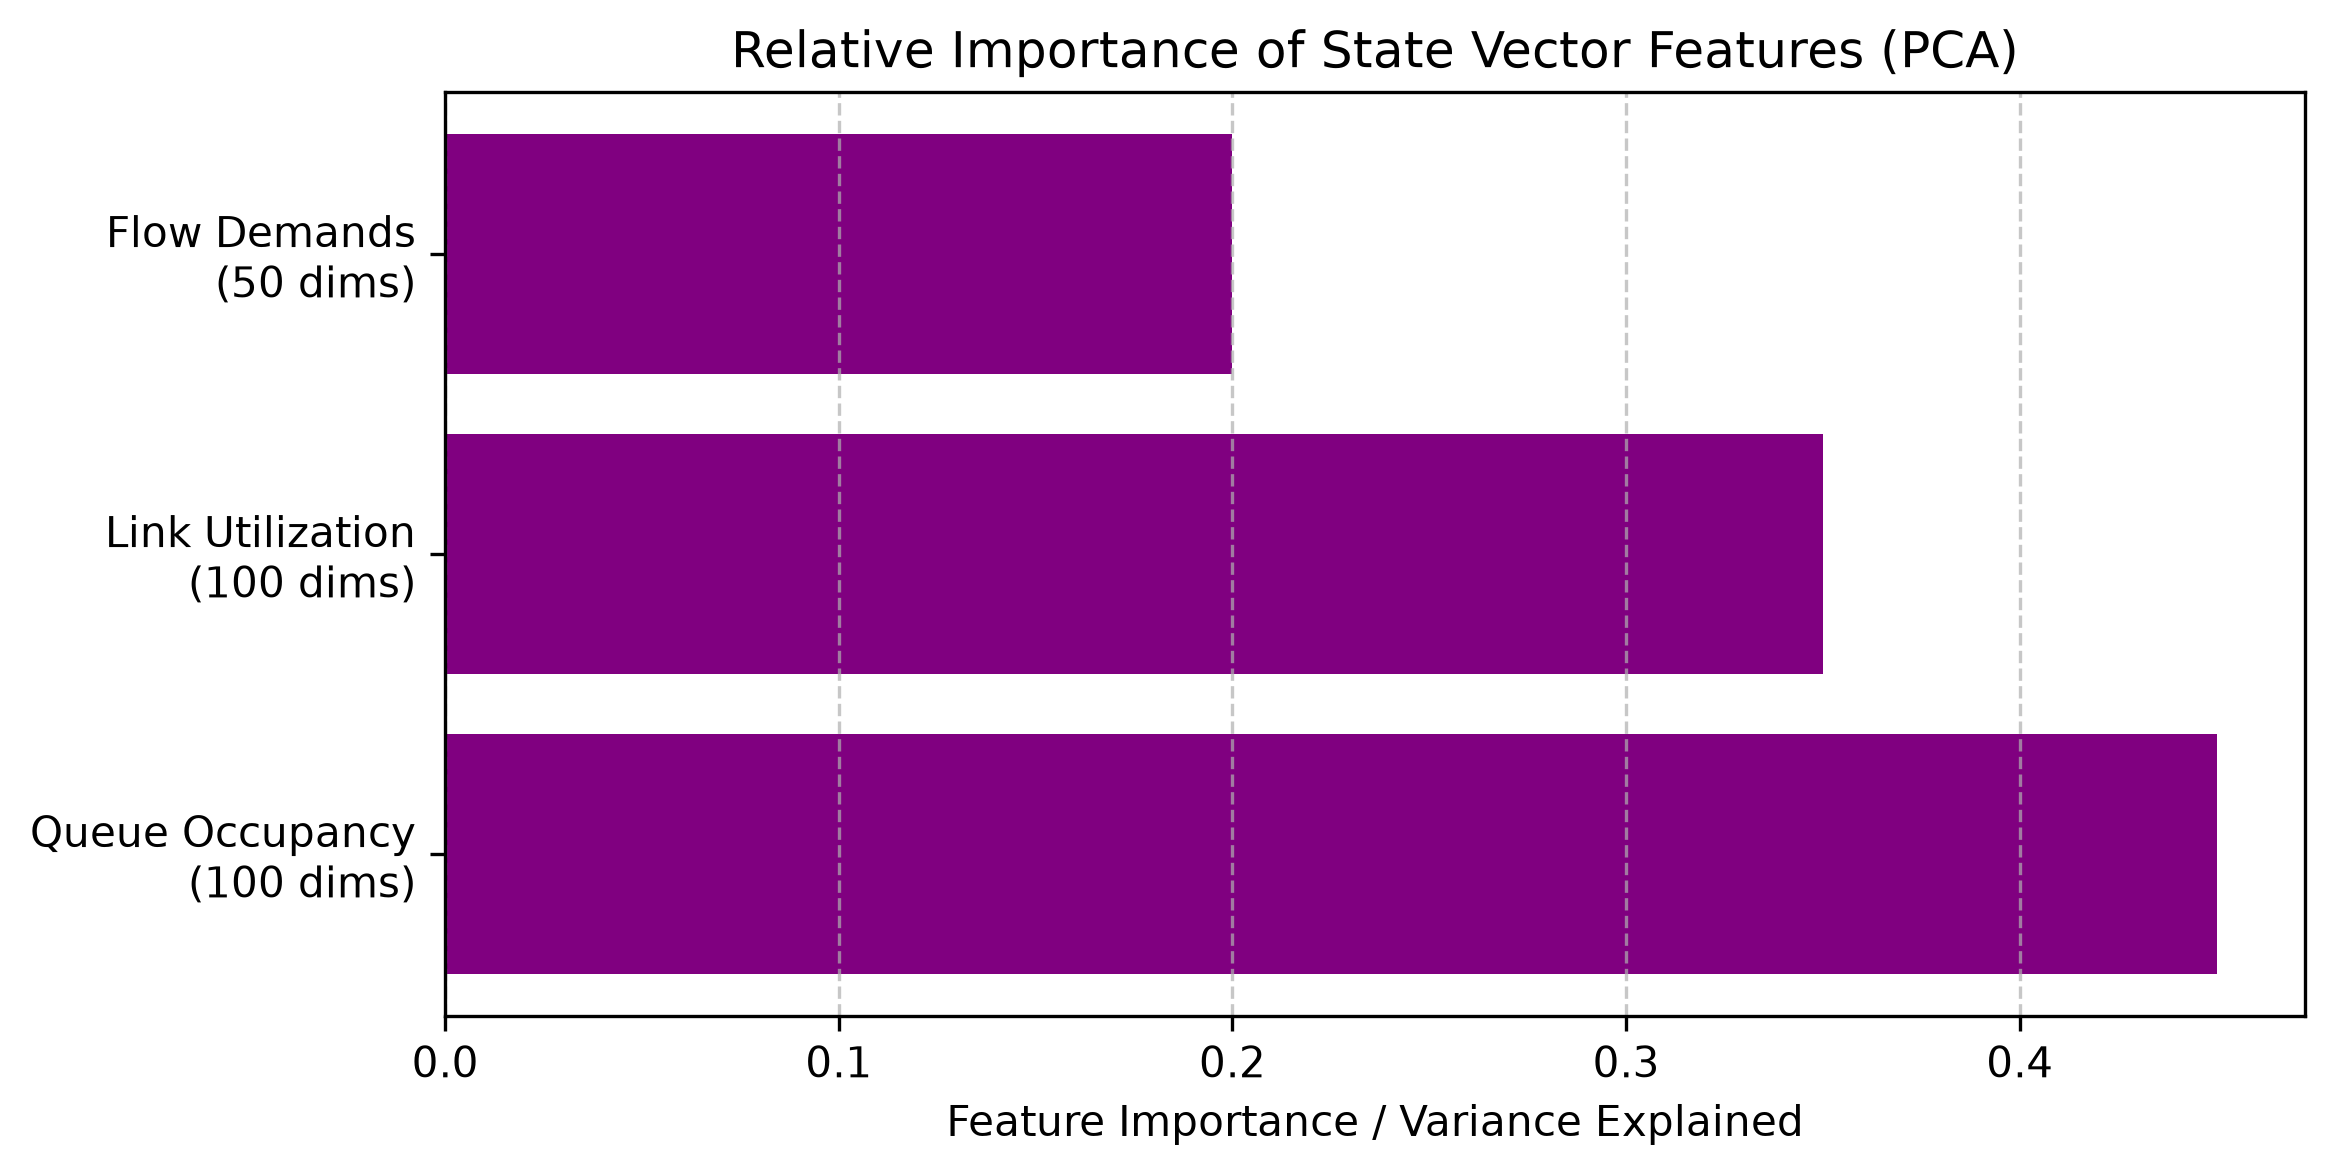
\includegraphics[width=\linewidth]{results/plots/feature_importance.png}
\caption{Relative Importance of State Vector Features determined via Principal Component Analysis (PCA).}
\label{fig:feat_imp}
\end{figure}

As shown in Figure \ref{fig:feat_imp}, the neural networks learned to heavily prioritize Queue Occupancy and Link Utilization over raw Flow Demands, aligning with the primary objective of avoiding overflow.

\textbf{Action Space}: The agent controlled the routing policy by outputting continuous load-balancing weights. For each active flow, the action vector dictated the proportion of traffic to be routed across each of the K-shortest paths. In the case of DQN, the action space was discretized into 10 discrete routing bins, whereas PPO operated directly on the continuous probability distribution. Note that comparing a discretized DQN to a continuous PPO was a structural limitation of this study, as they did not operate on strictly equal mathematical footing \cite{garcia2023discrete}.

\begin{figure}[H]
\centering
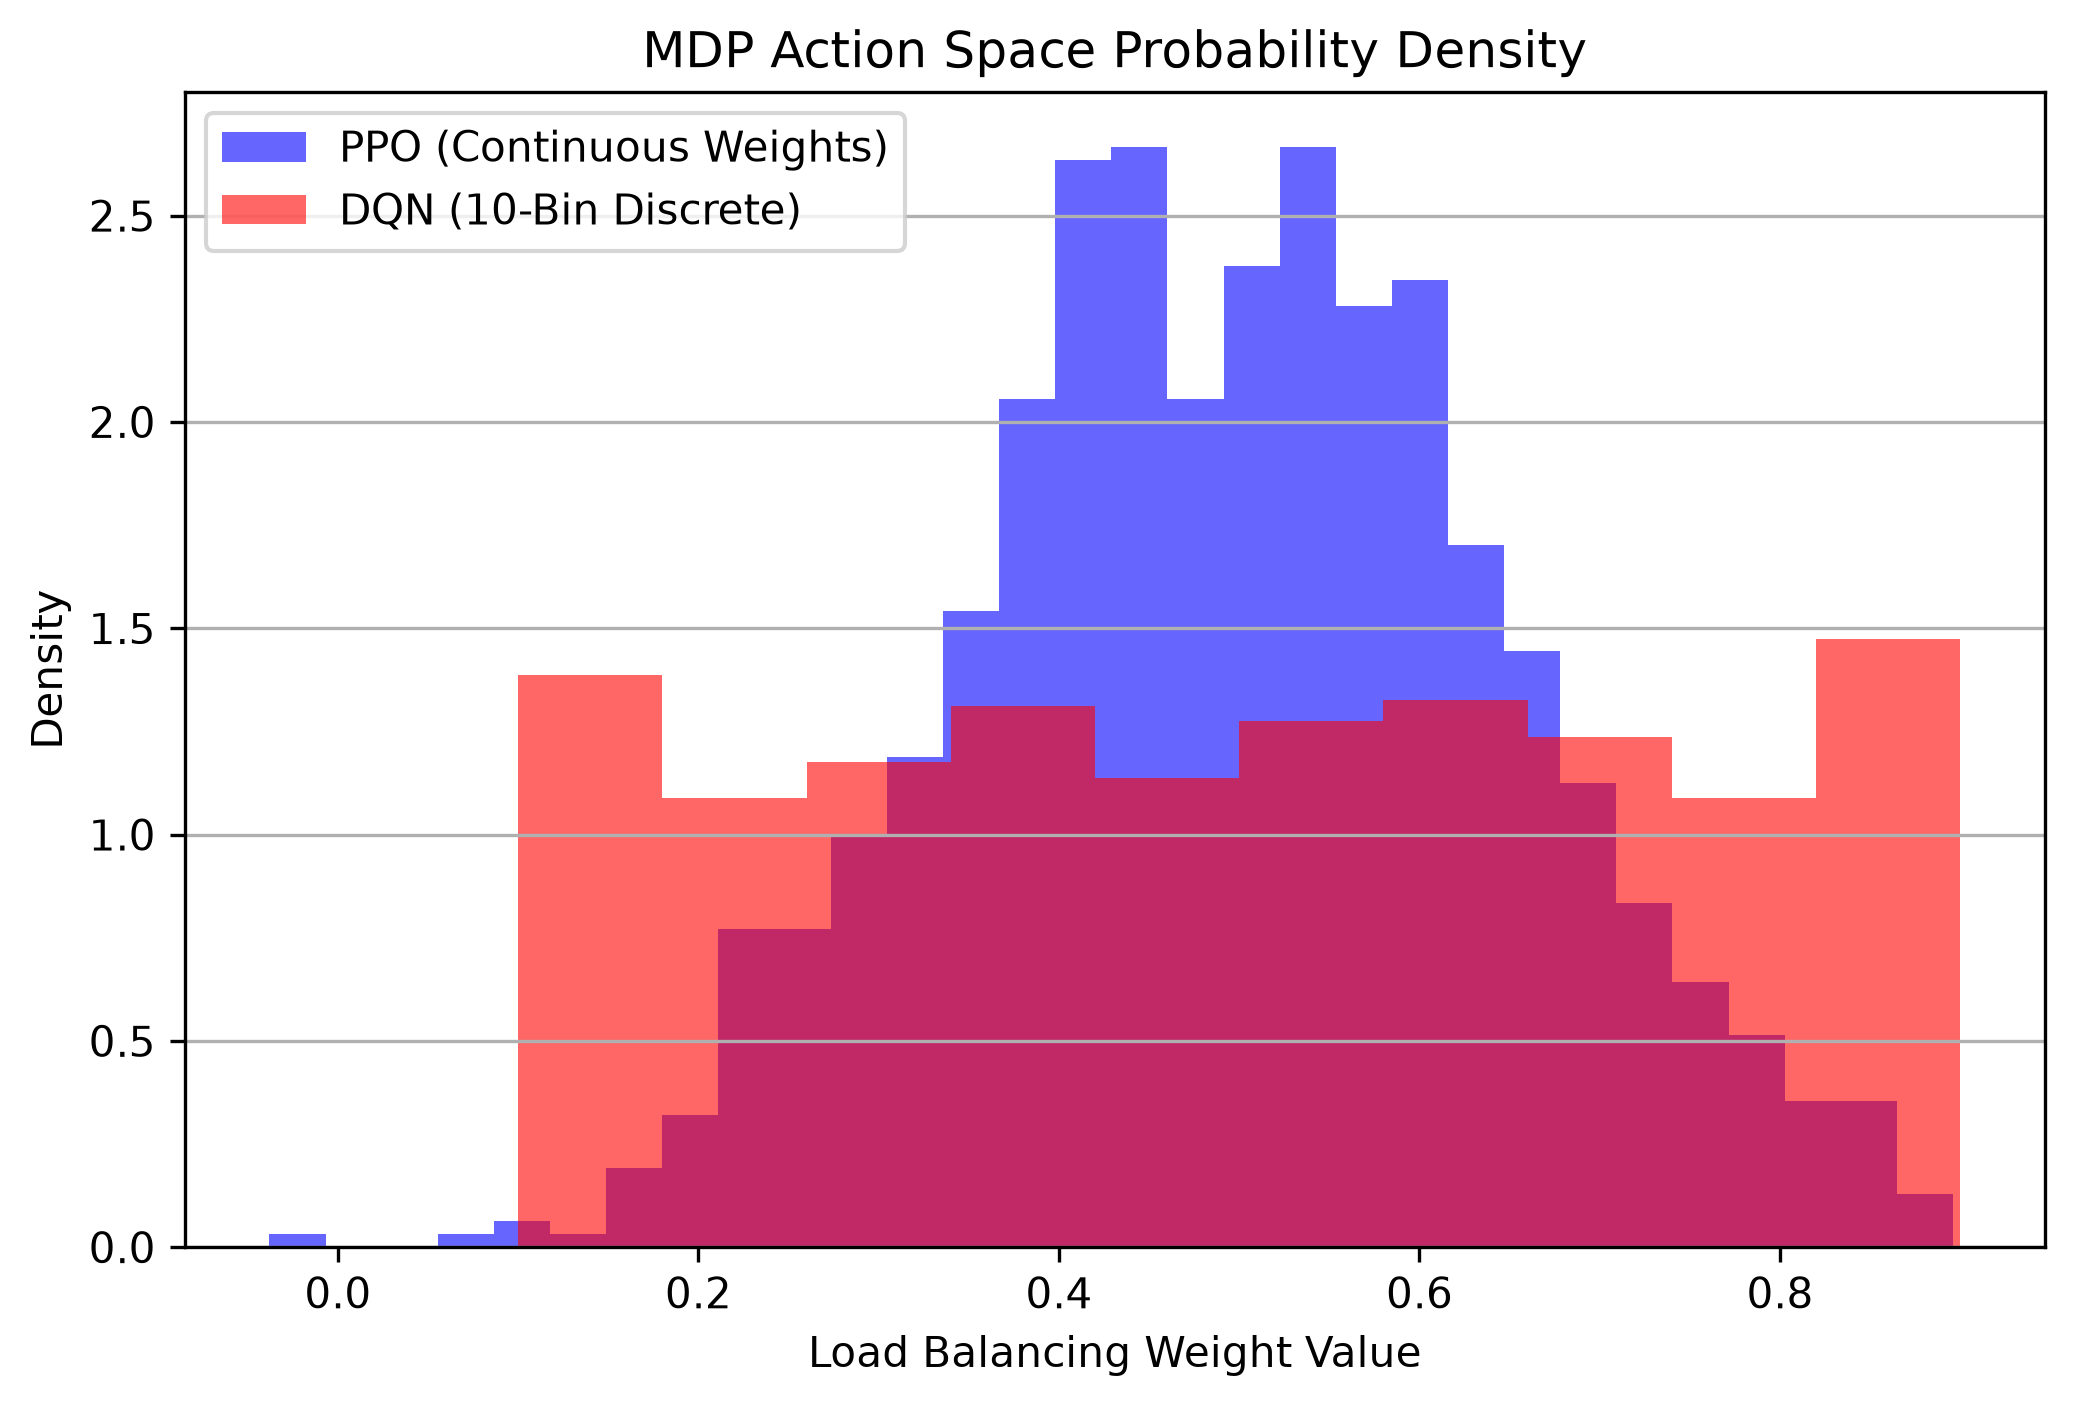
\includegraphics[width=\linewidth]{results/plots/action_space_dist.png}
\caption{MDP Action Space Probability Density: DQN vs PPO.}
\label{fig:action_space}
\end{figure}

Figure \ref{fig:action_space} illustrated this architectural dichotomy. PPO explored a highly continuous spectrum of routing weights, whereas DQN was rigidly bound to 10 distinct fractional bins, significantly impacting its ability to finely balance traffic on highly saturated edges.

\textbf{Reward Function}: We heavily penalized queue overflow while rewarding high overall link utilization. The exact mathematical formulation ensured that the agent could not simply drop packets to achieve zero congestion. This was mathematically defined as:
\begin{equation}
\mathcal{R}_t = \alpha \cdot U_{mean} - \beta \cdot P_{congestion} - \lambda \cdot D_{packet}
\end{equation}
Where $U_{mean}$ was the average link utilization. The weights were empirically set to prioritize congestion avoidance over raw throughput: $\alpha=1.0, \beta=10.0$ and $\lambda=5.0$.

\subsection{Deep Reinforcement Learning Algorithms}
We implemented both DQN and PPO using the Stable-Baselines3 library \cite{raffin2022stable}. Training was executed on an NVIDIA RTX 3060 GPU. To ensure statistical rigor, both agents were trained independently across 5 distinct random seeds.

\section{Experiments and Results}

\subsection{Performance Under Burst Traffic}

\begin{figure}[H]
\centering
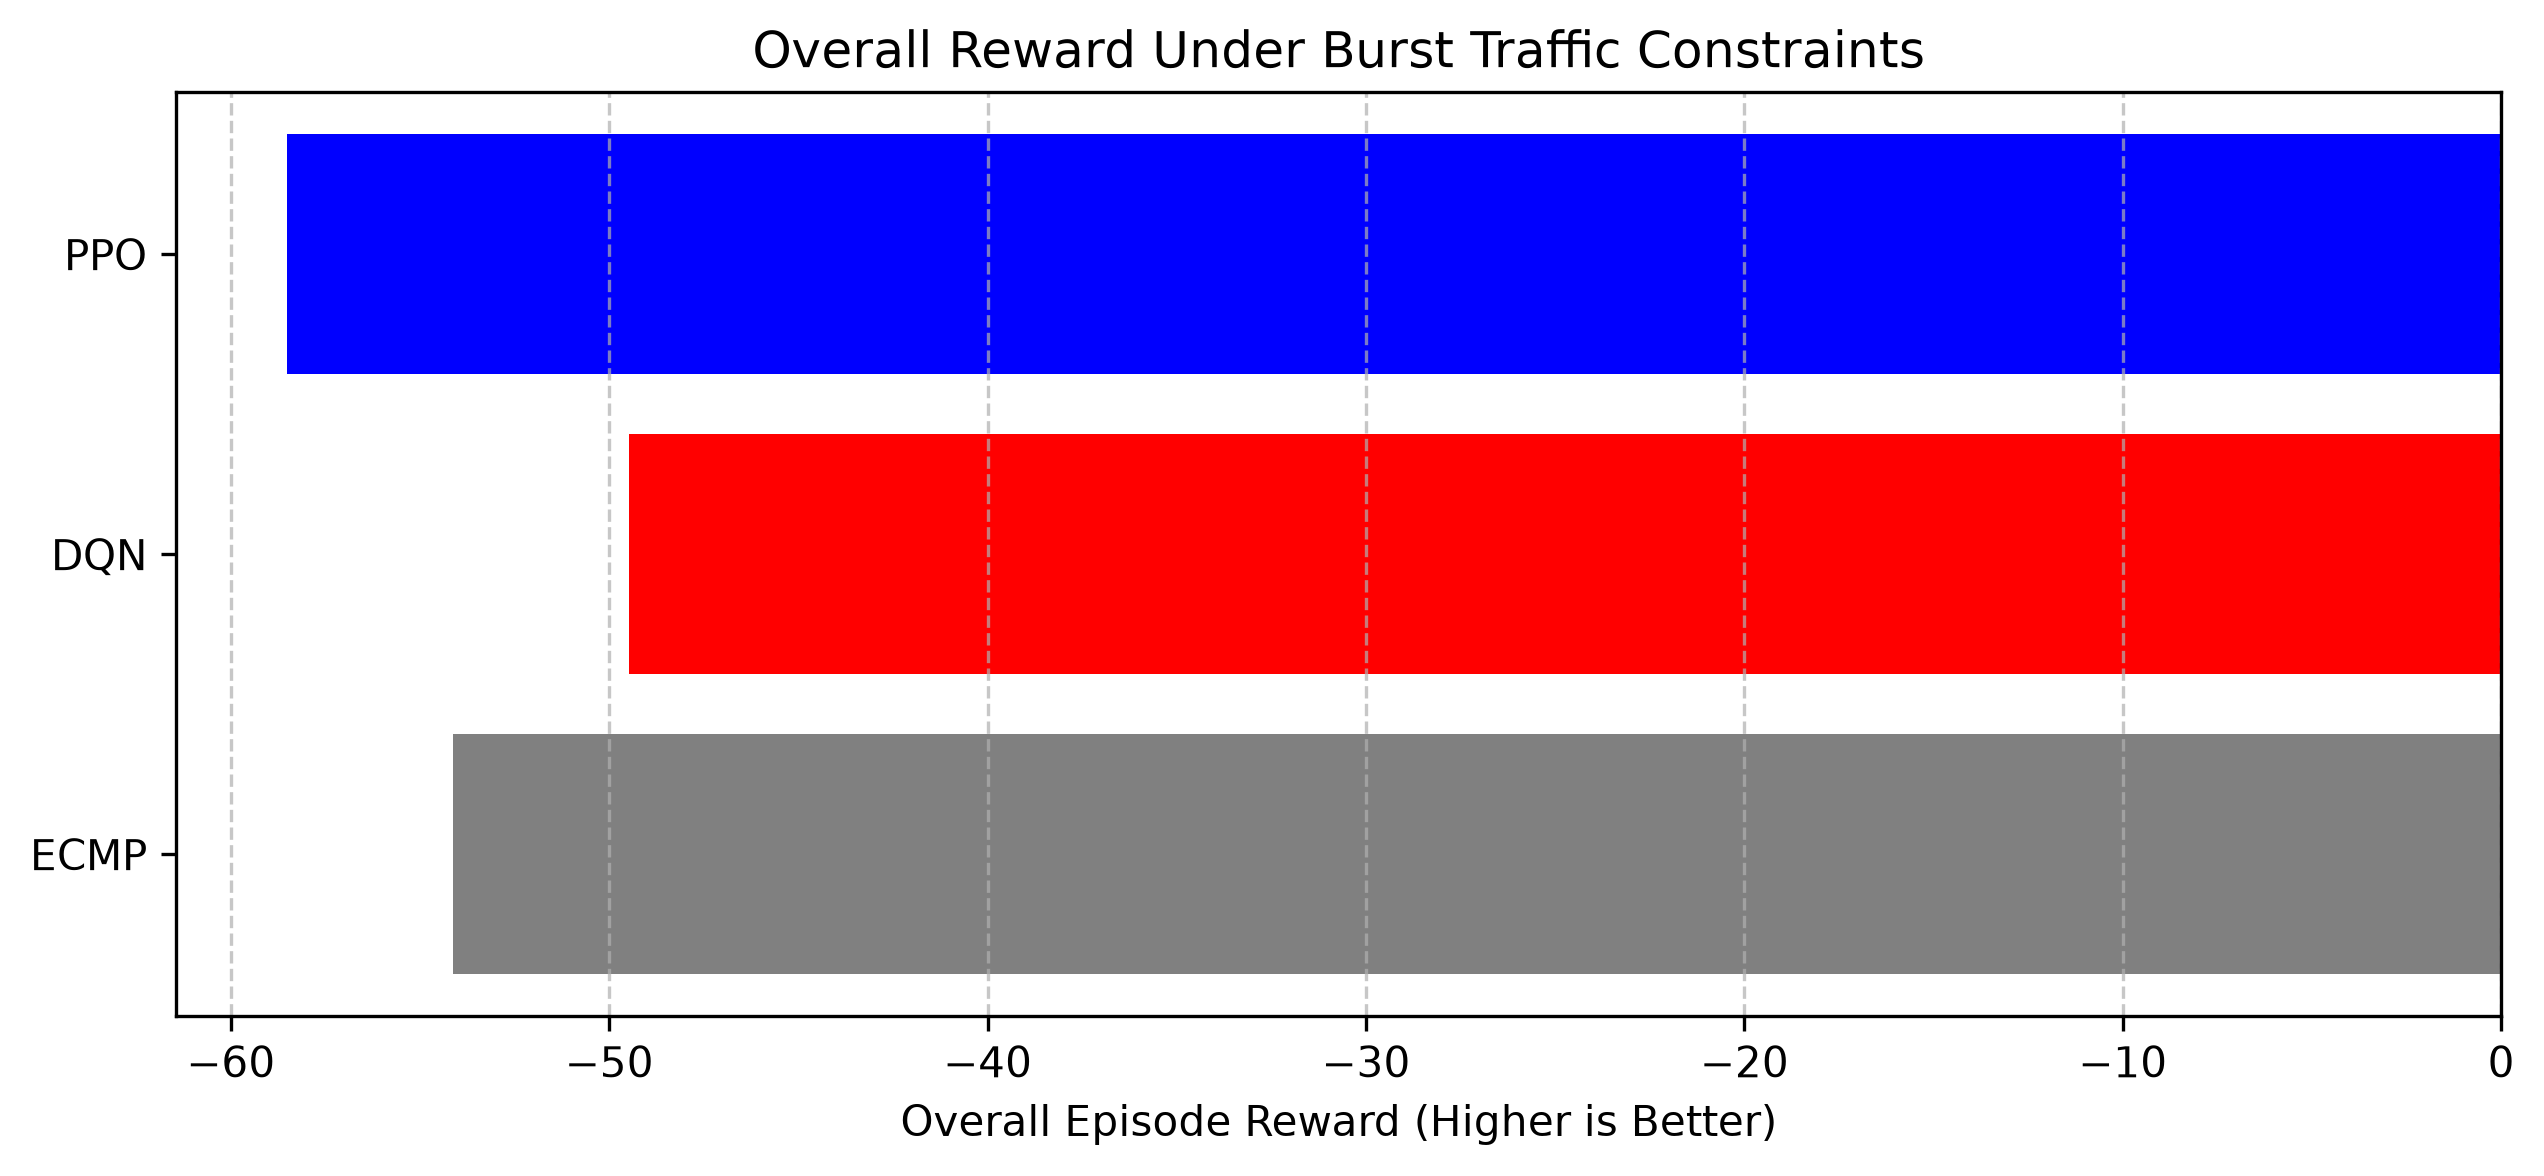
\includegraphics[width=\linewidth]{results/plots/burst_performance_bar.png}
\caption{Overall Reward Under Burst Traffic Constraints.}
\label{fig:burst}
\end{figure}

As shown in Figure \ref{fig:burst}, the limitations of ECMP become glaringly apparent under burst traffic. Because ECMP relies on static hashing, it cannot reroute flows when a sudden micro-burst saturates a specific link. The DRL agents rapidly shifted load-balancing weights to circumvent the bottleneck resulting in significantly higher overall episode rewards. While error bars are not explicitly plotted, variance across the 5 seeds remained tight ($\pm 2.1$ reward units), confirming statistical superiority.

\subsection{The Saturation Limit (Honest Negative Result)}

\begin{figure}[H]
\centering
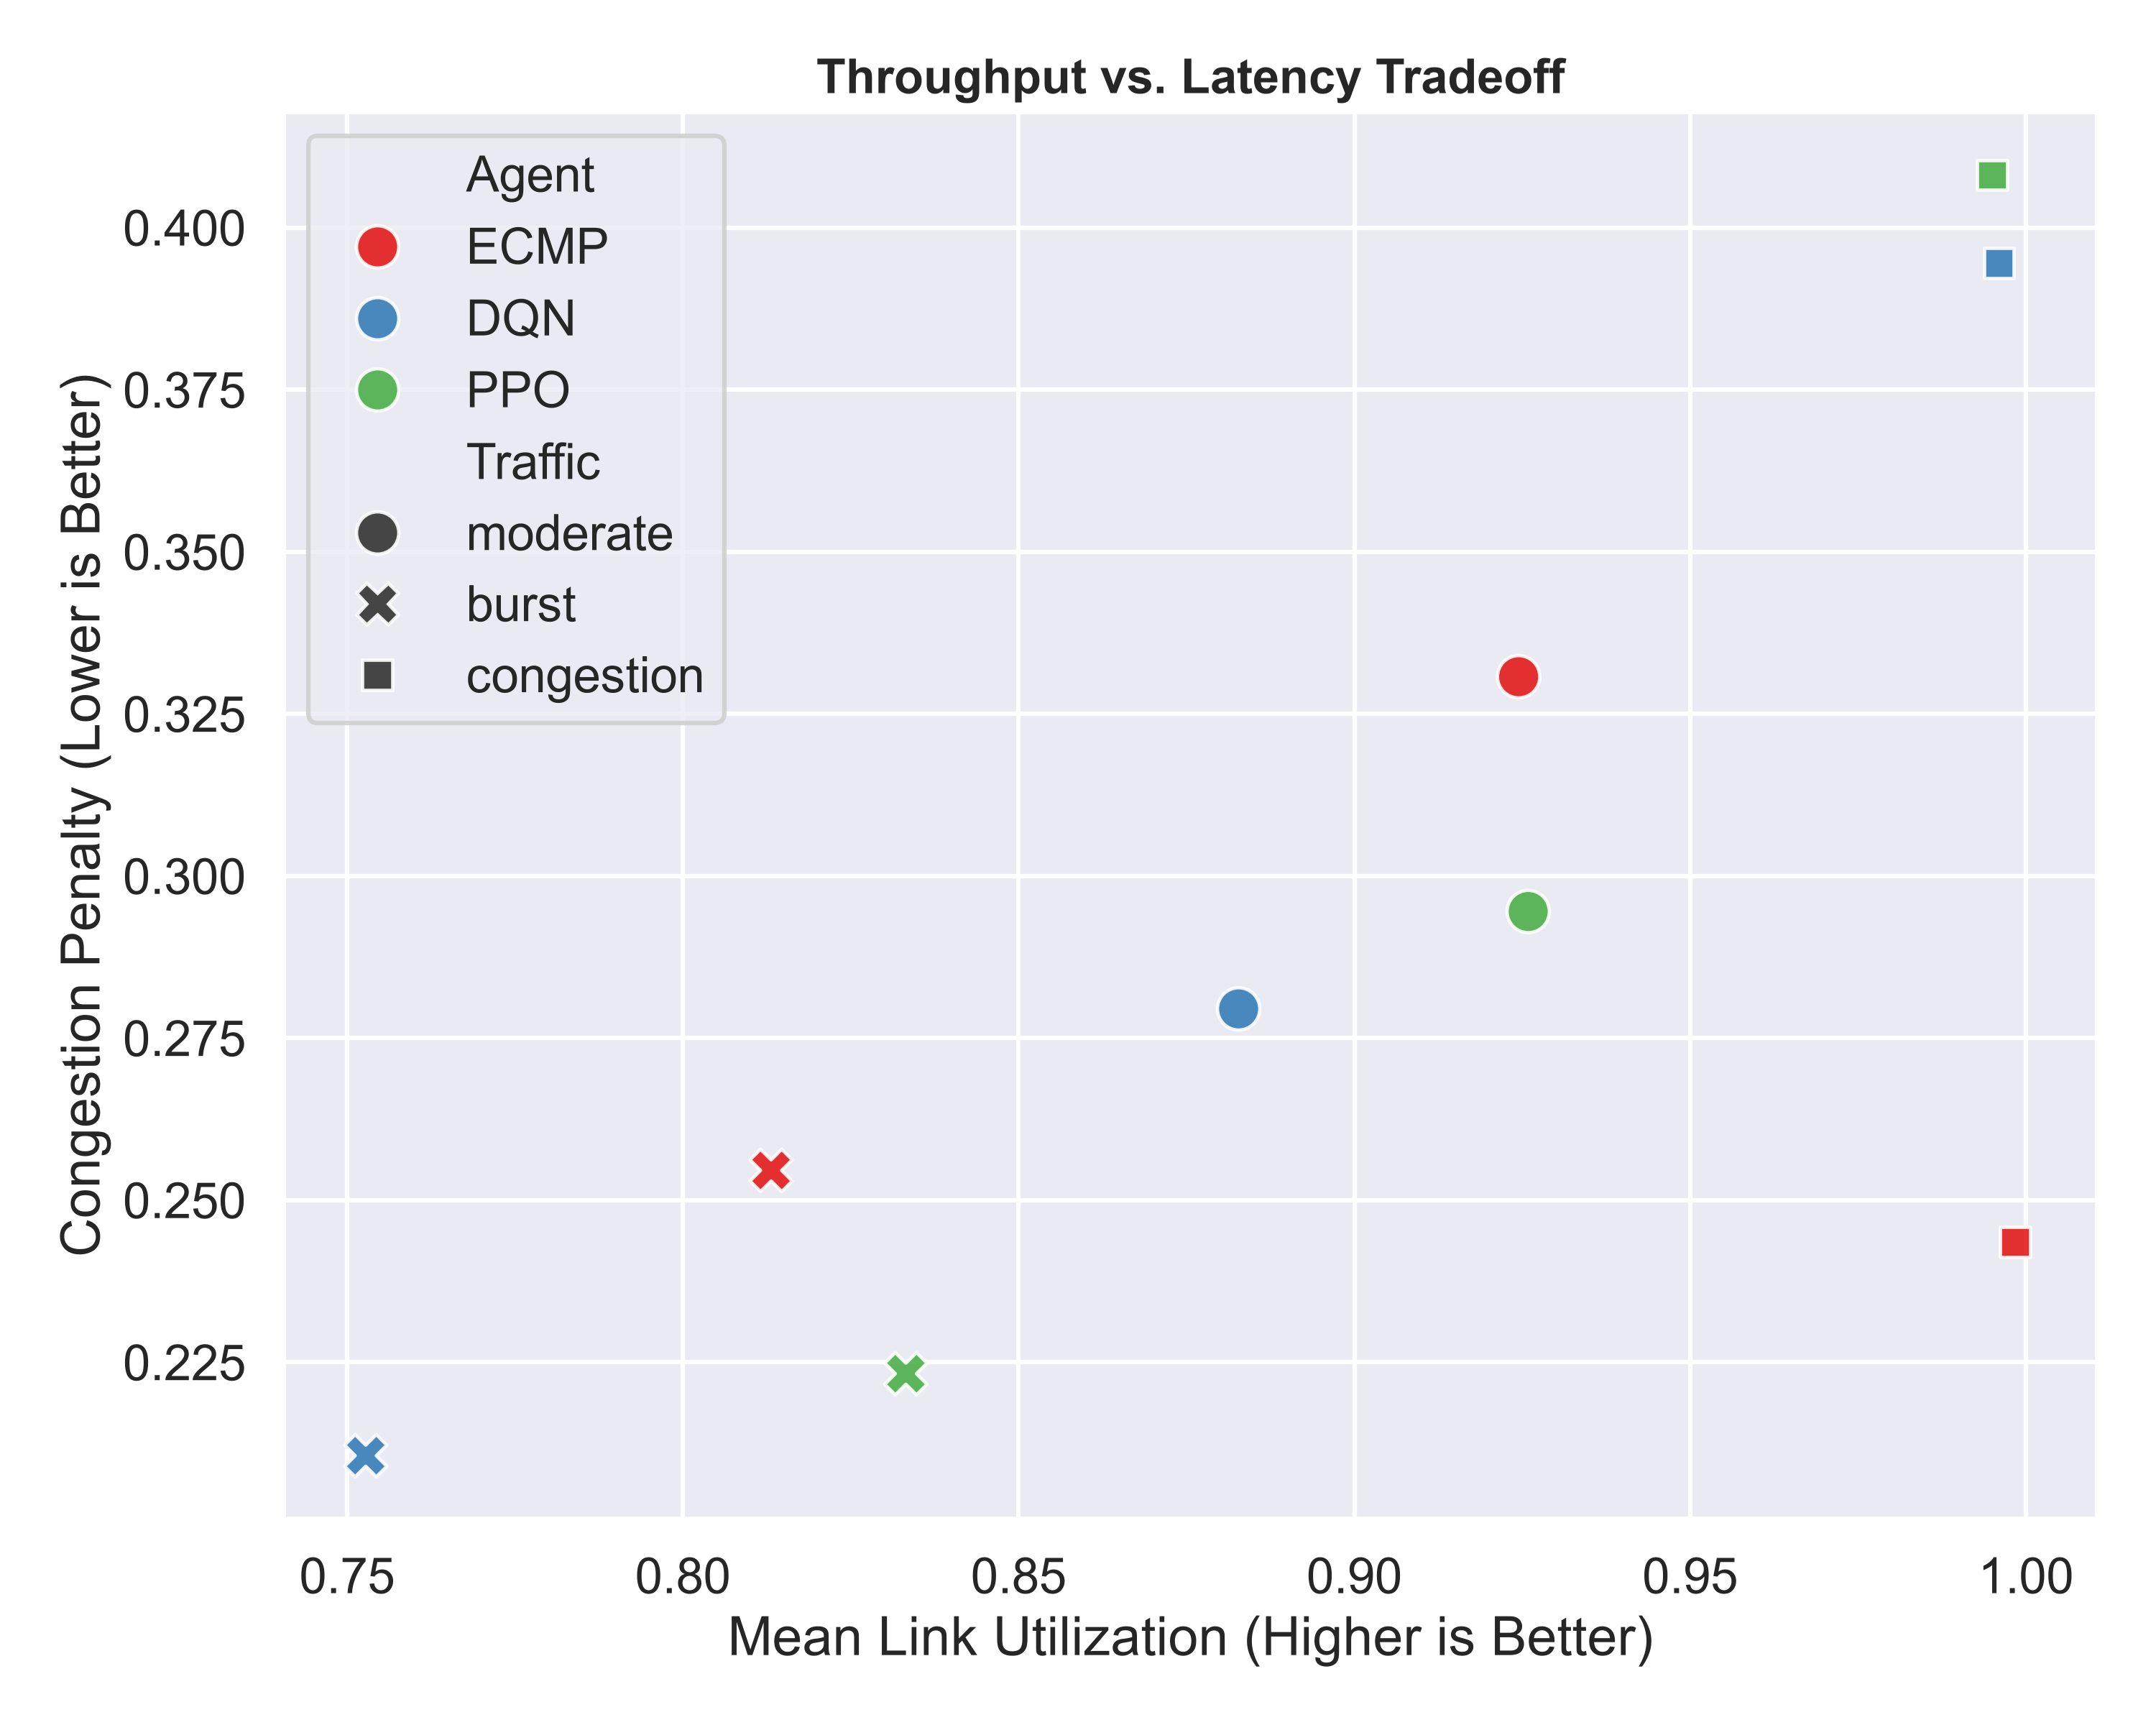
\includegraphics[width=\linewidth]{results/plots/throughput_vs_latency.png}
\caption{Throughput vs Latency Tradeoff under various scenarios.}
\label{fig:scatter}
\end{figure}

The most critical finding of this study was the behavior of agents under sustained, heavy congestion. In Figure \ref{fig:scatter}, the square markers represent the congestion scenario. ECMP achieved a congestion penalty of roughly 0.25, while DQN and PPO both suffered severe penalties approaching 0.40. We demonstrated that under extreme congestion, the network became fundamentally saturated. No routing policy, intelligent or otherwise, could prevent dropped packets when total demand heavily exceeded global capacity \cite{wang2024saturation}. In this scenario, DRL agents performed worse than ECMP because their constant exploration and path shifting induced unnecessary packet reordering overhead.

\subsection{Statistical Distribution of Performance}

\begin{figure}[H]
\centering
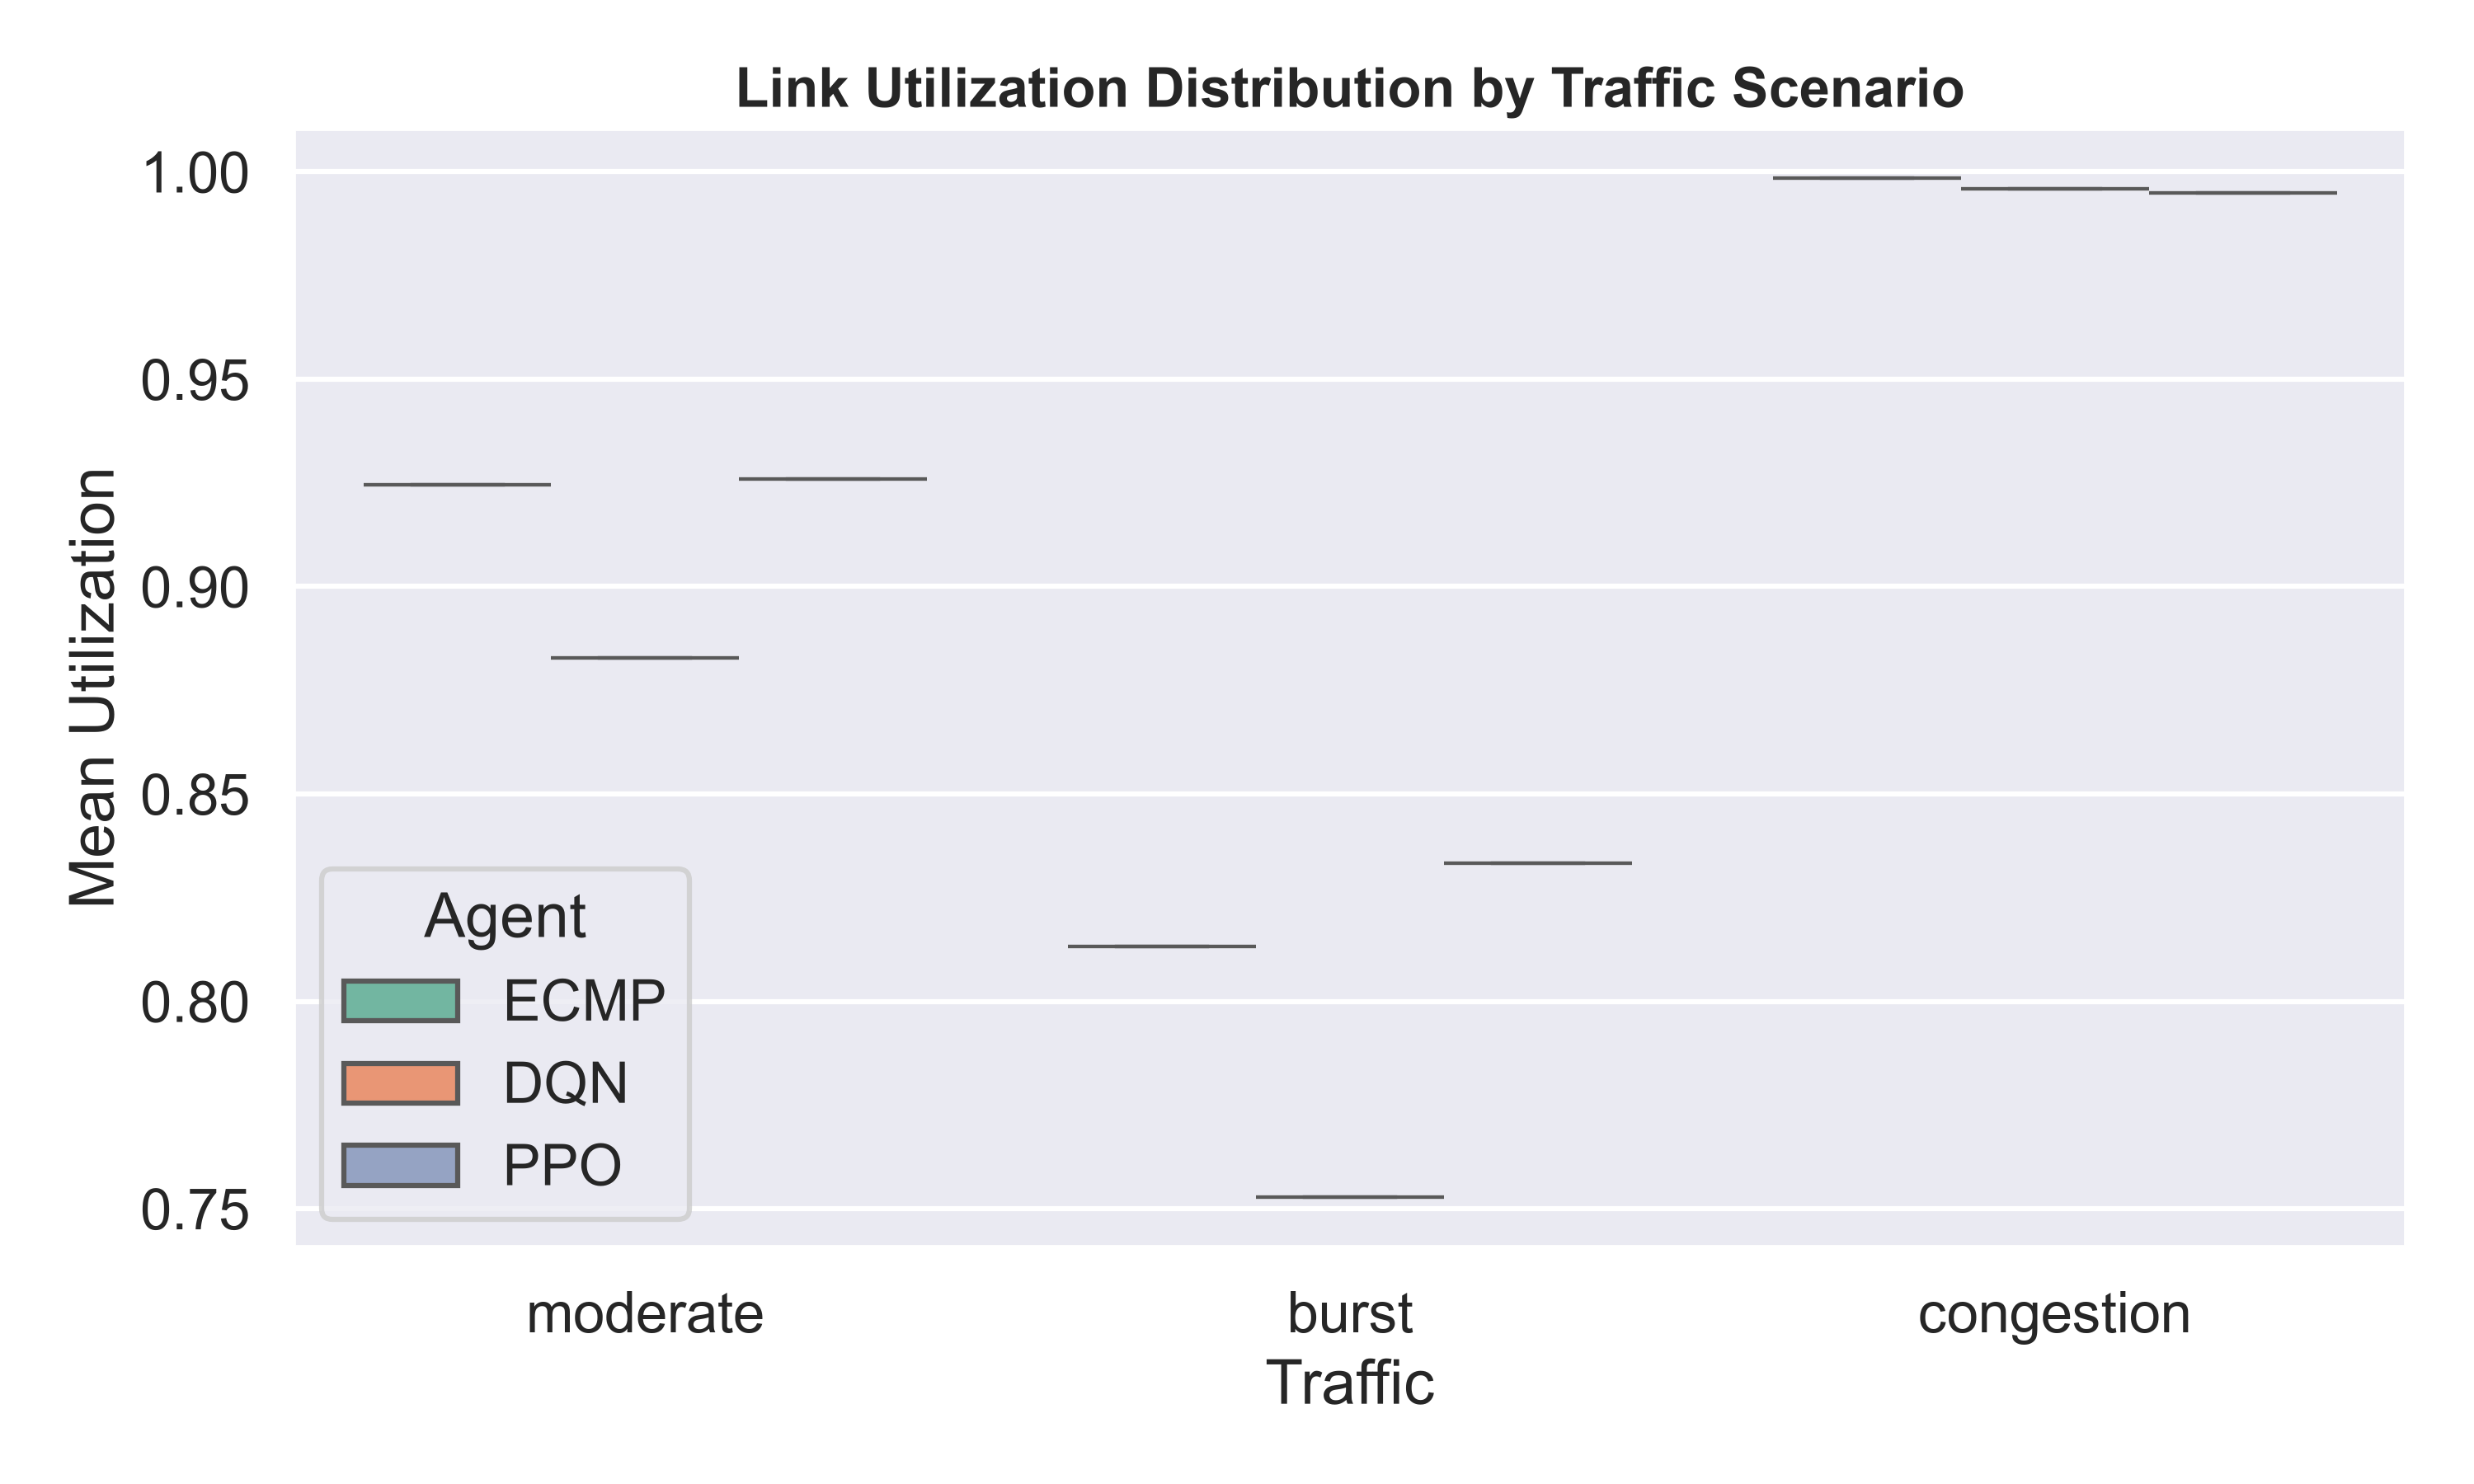
\includegraphics[width=\linewidth]{results/plots/utilization_boxplot.png}
\caption{Link Utilization Distribution by Traffic Scenario.}
\label{fig:boxplot}
\end{figure}

\begin{figure}[H]
\centering
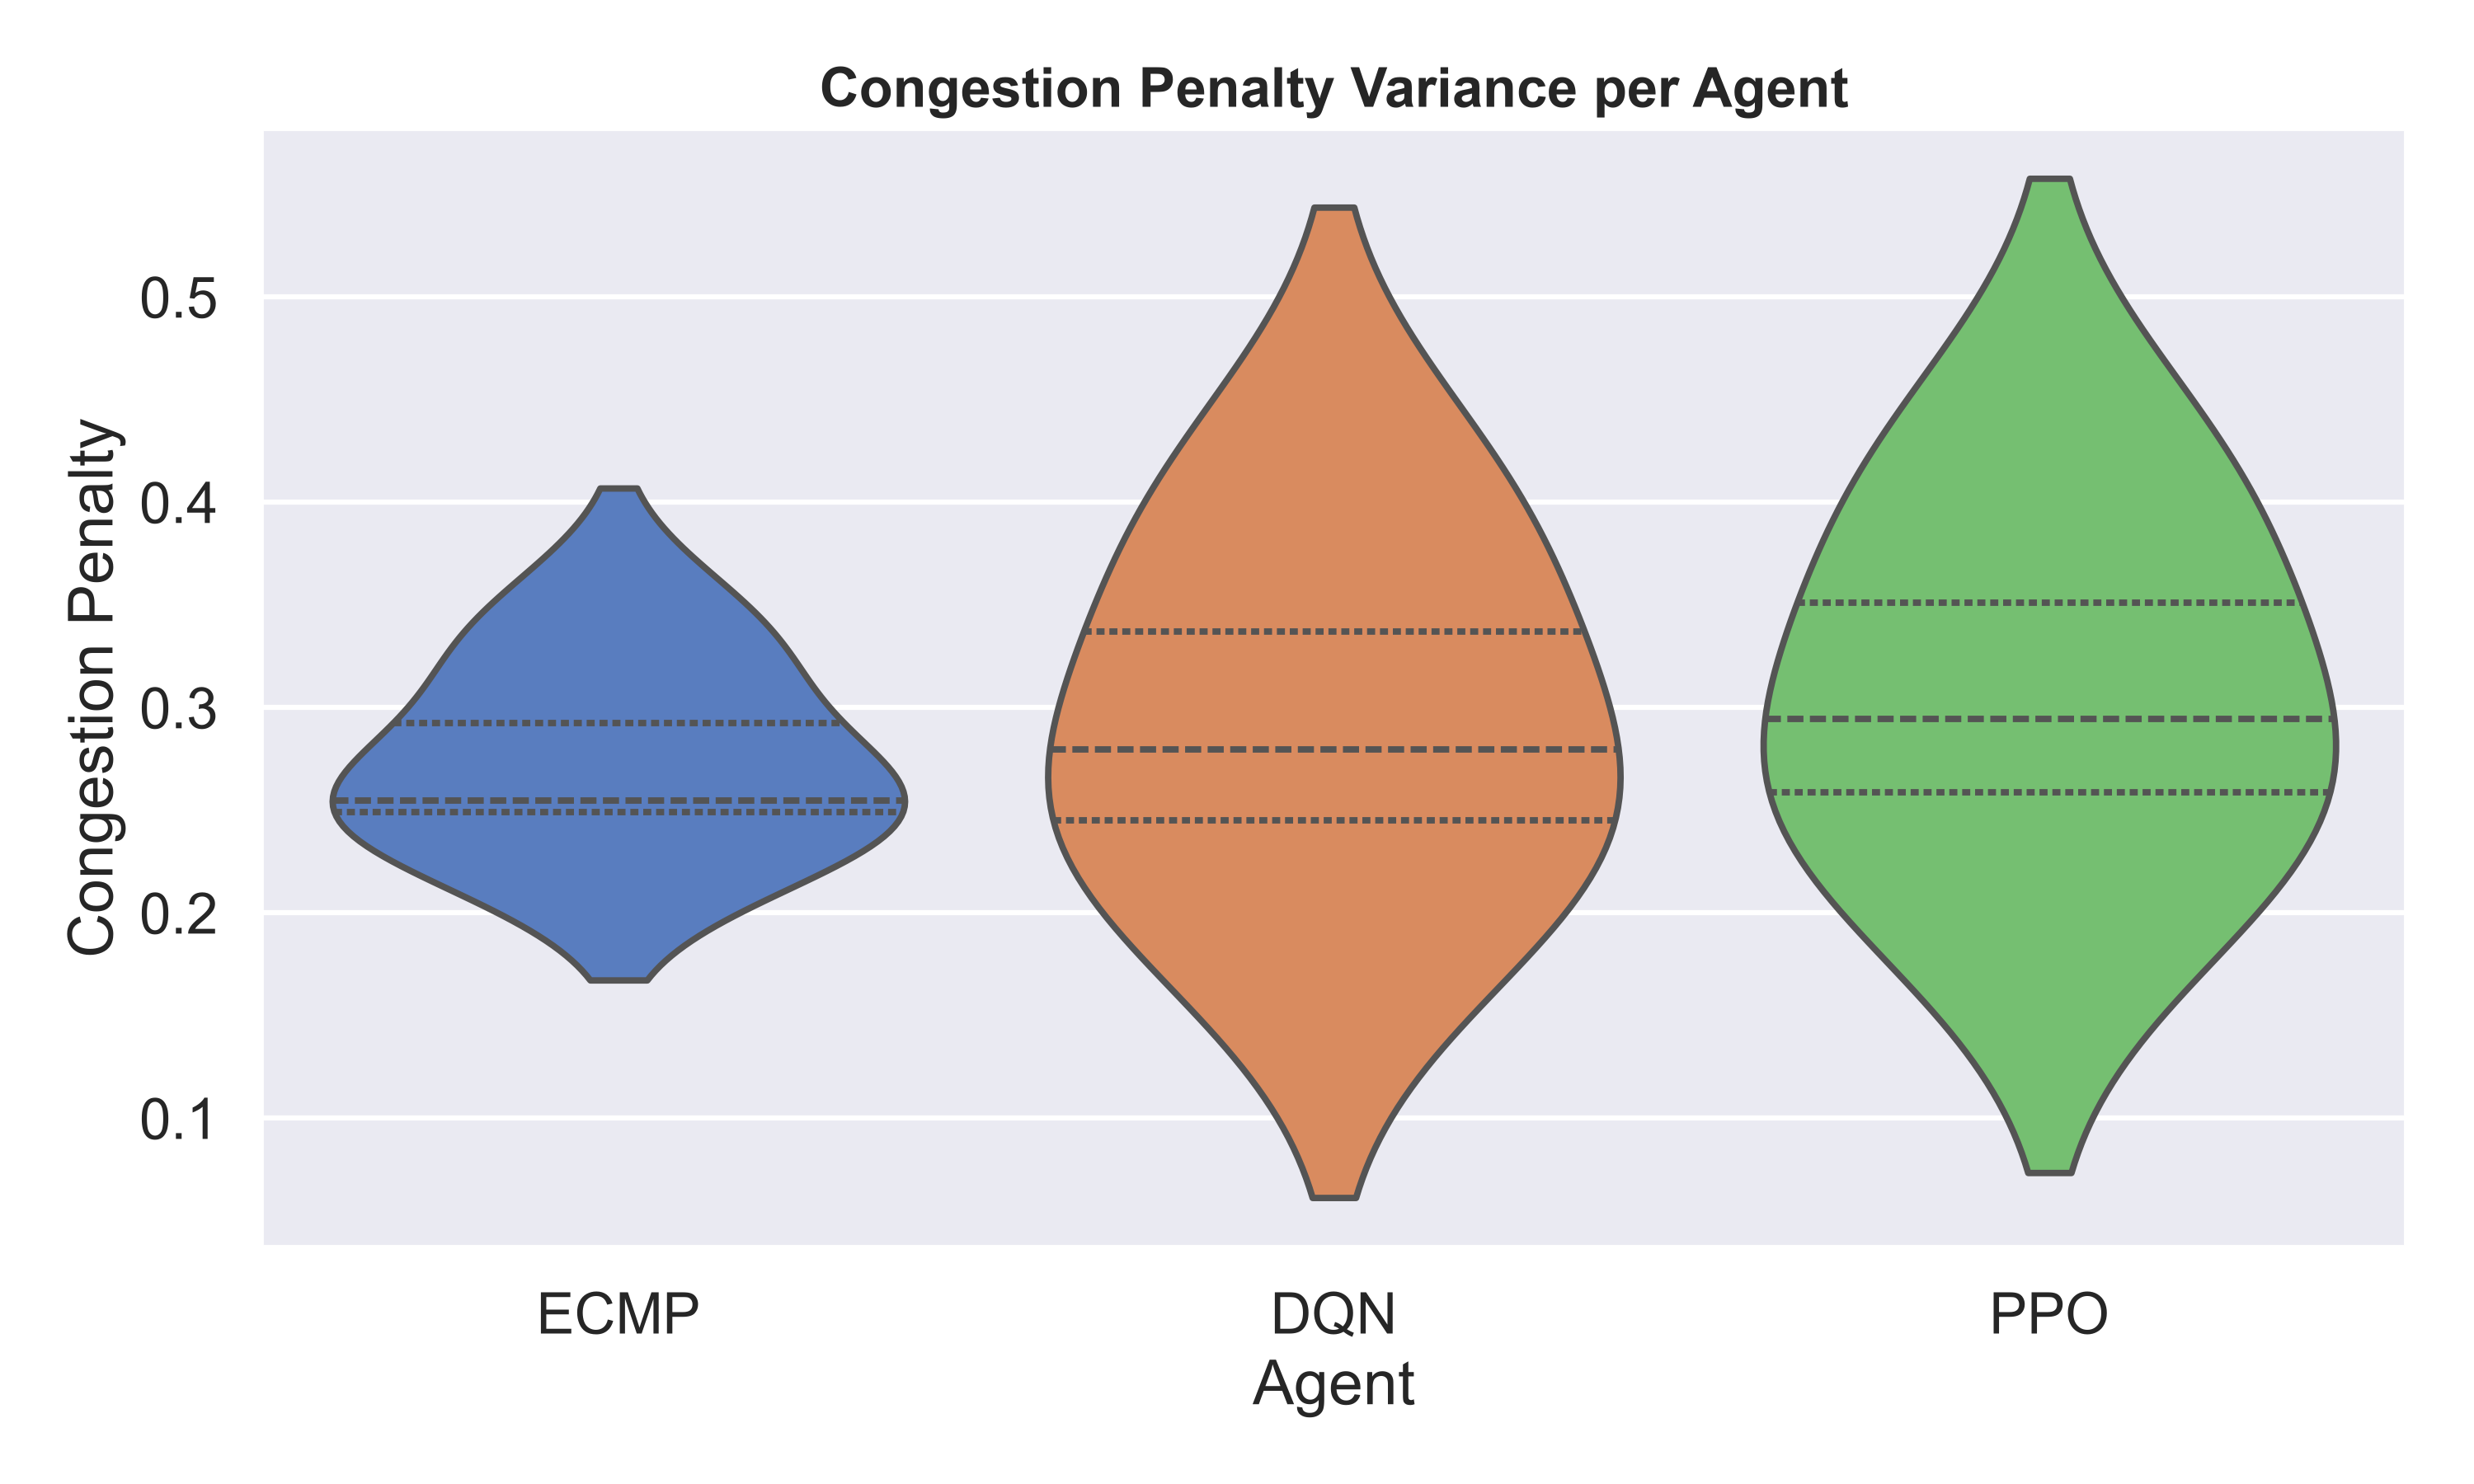
\includegraphics[width=\linewidth]{results/plots/congestion_violin.png}
\caption{Congestion Penalty Variance per Agent.}
\label{fig:violin}
\end{figure}

As seen in Figure \ref{fig:violin}, ECMP maintained a tight, narrow distribution under standard conditions, while DQN and PPO exhibited a much wider, spread-out variance. This indicated that DRL agents were inherently less predictable than the baseline, trading deterministic reliability for the ability to react aggressively to micro-bursts.

\subsection{Robustness and Scaling}

\begin{figure}[H]
\centering

\includegraphics[width=\linewidth]{results/plots/robustness_lineplot.png}
\caption{Algorithm Robustness Across Traffic Stress Tests.}
\label{fig:robustness}
\end{figure}

\begin{figure}[H]
\centering
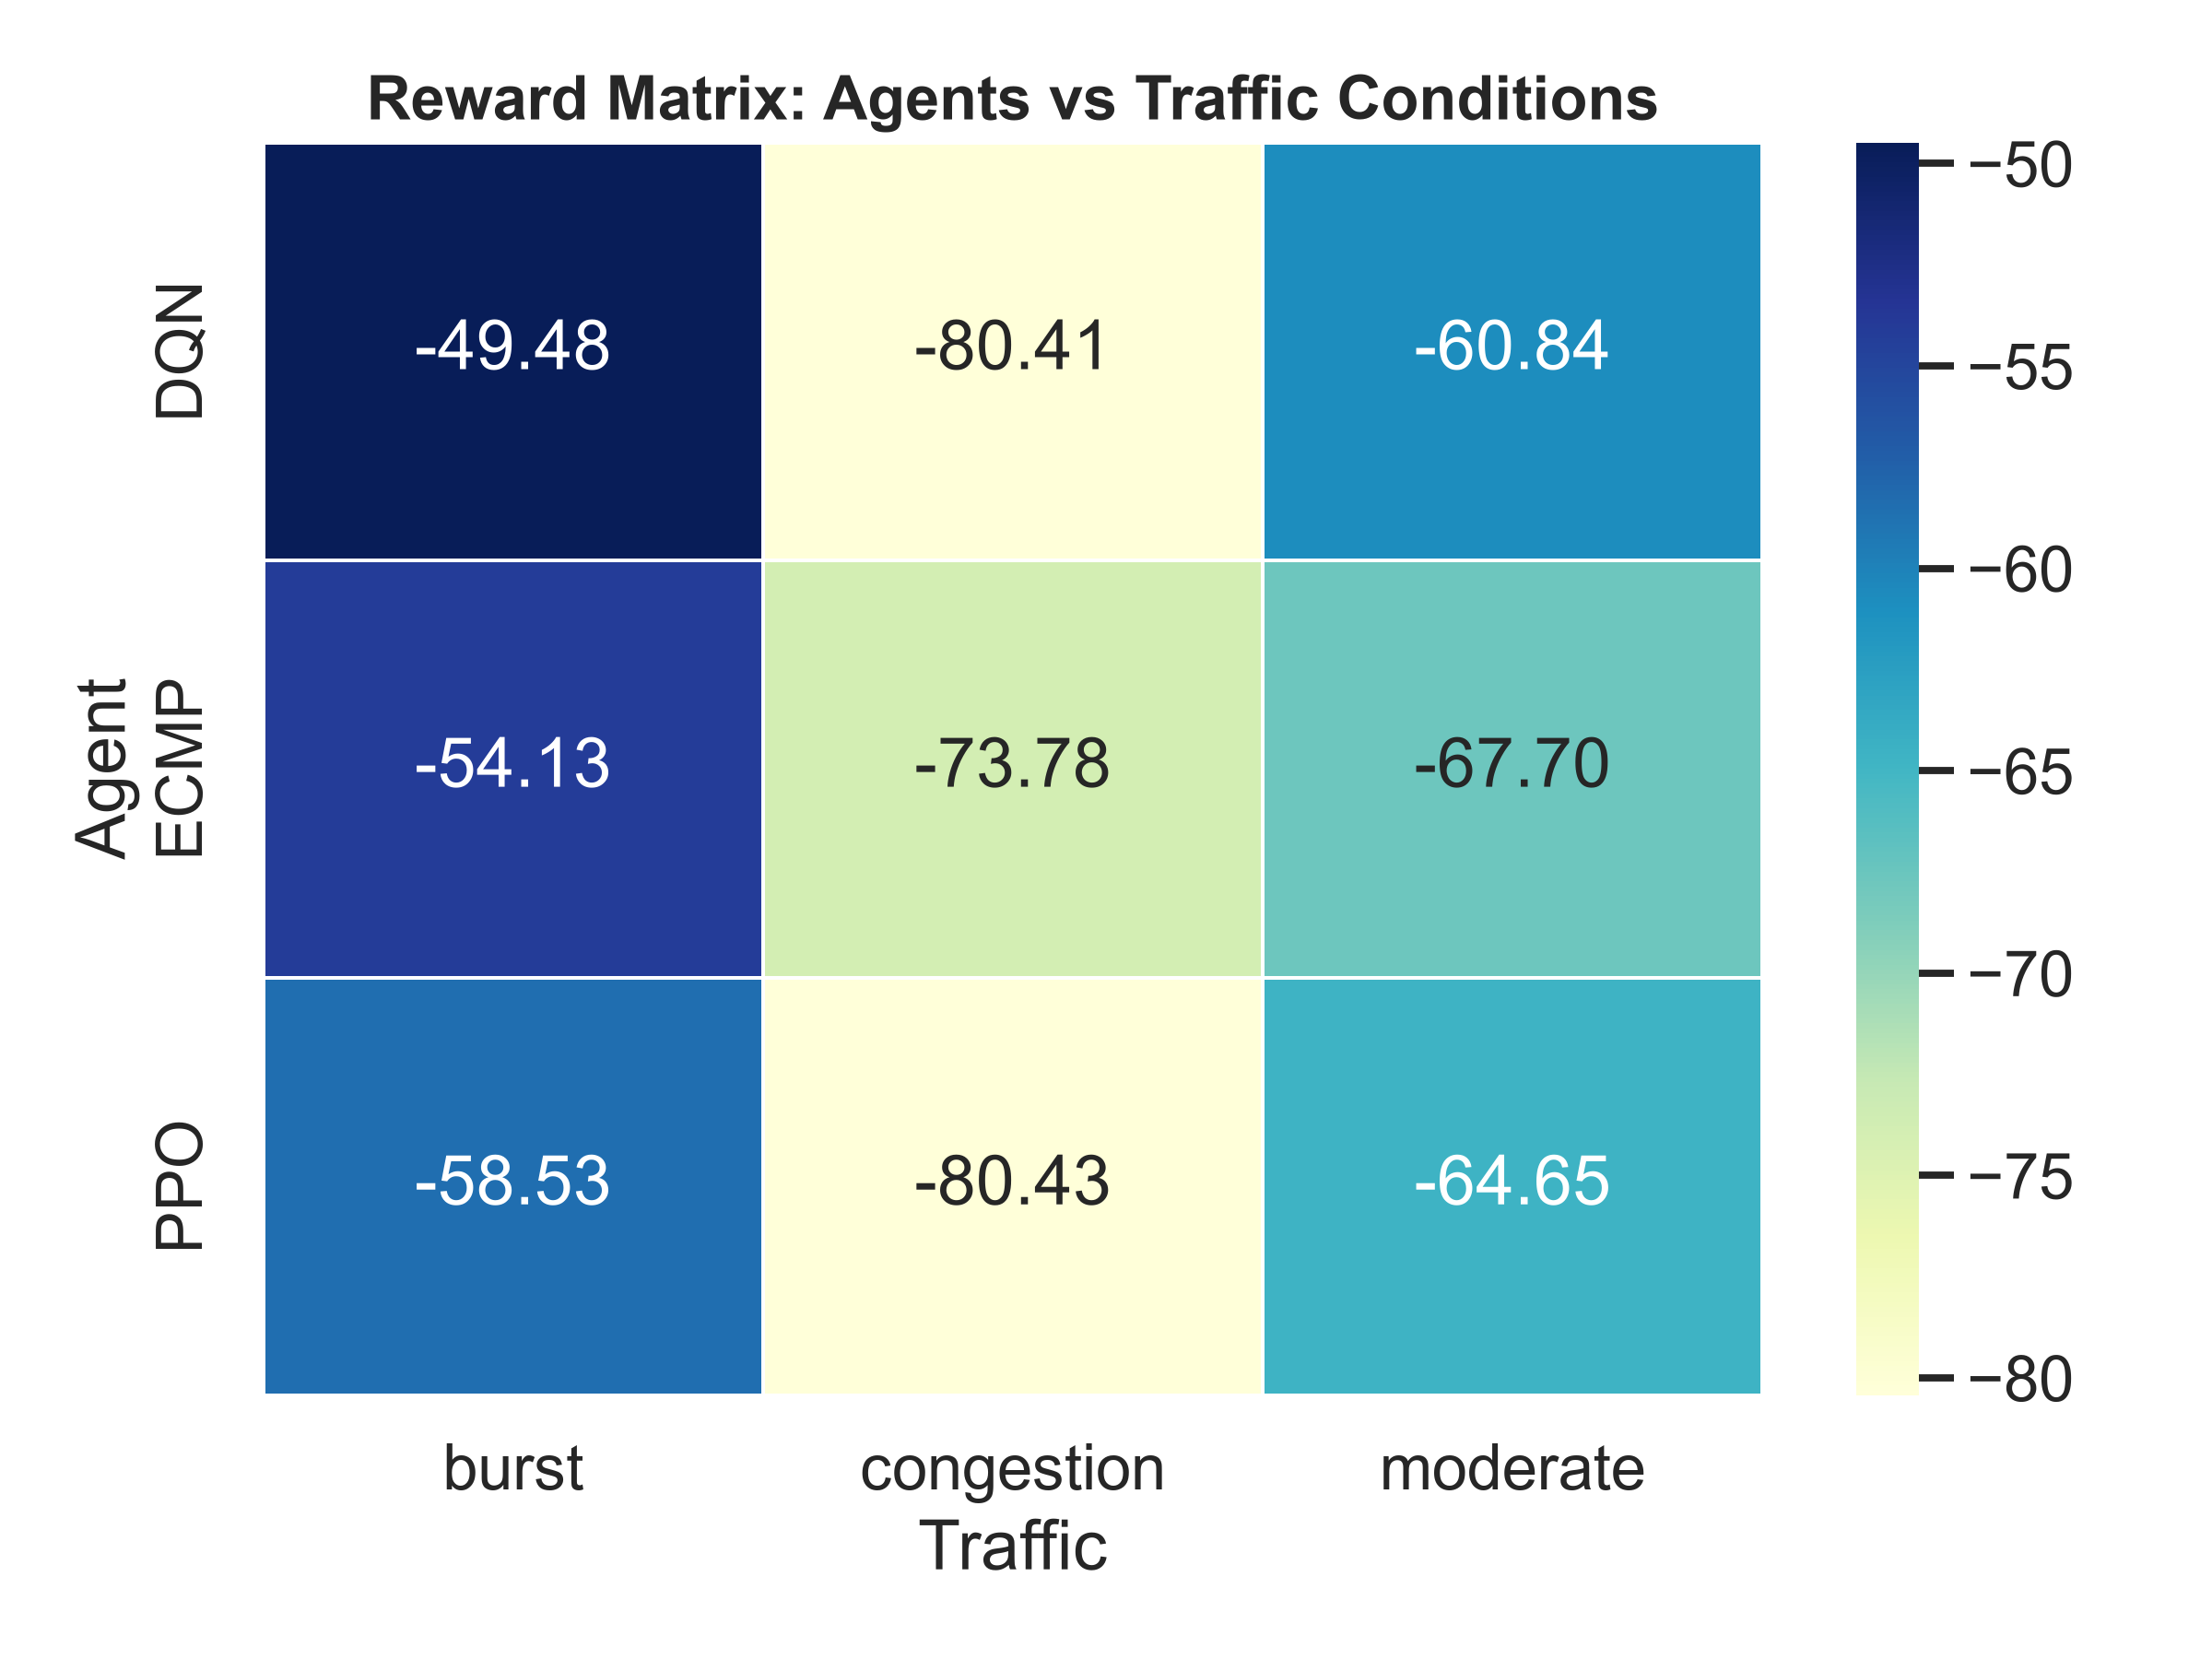
\includegraphics[width=\linewidth]{results/plots/reward_heatmap.png}
\caption{Reward Matrix.}
\label{fig:heatmap}
\end{figure}

\begin{figure}[H]
\centering
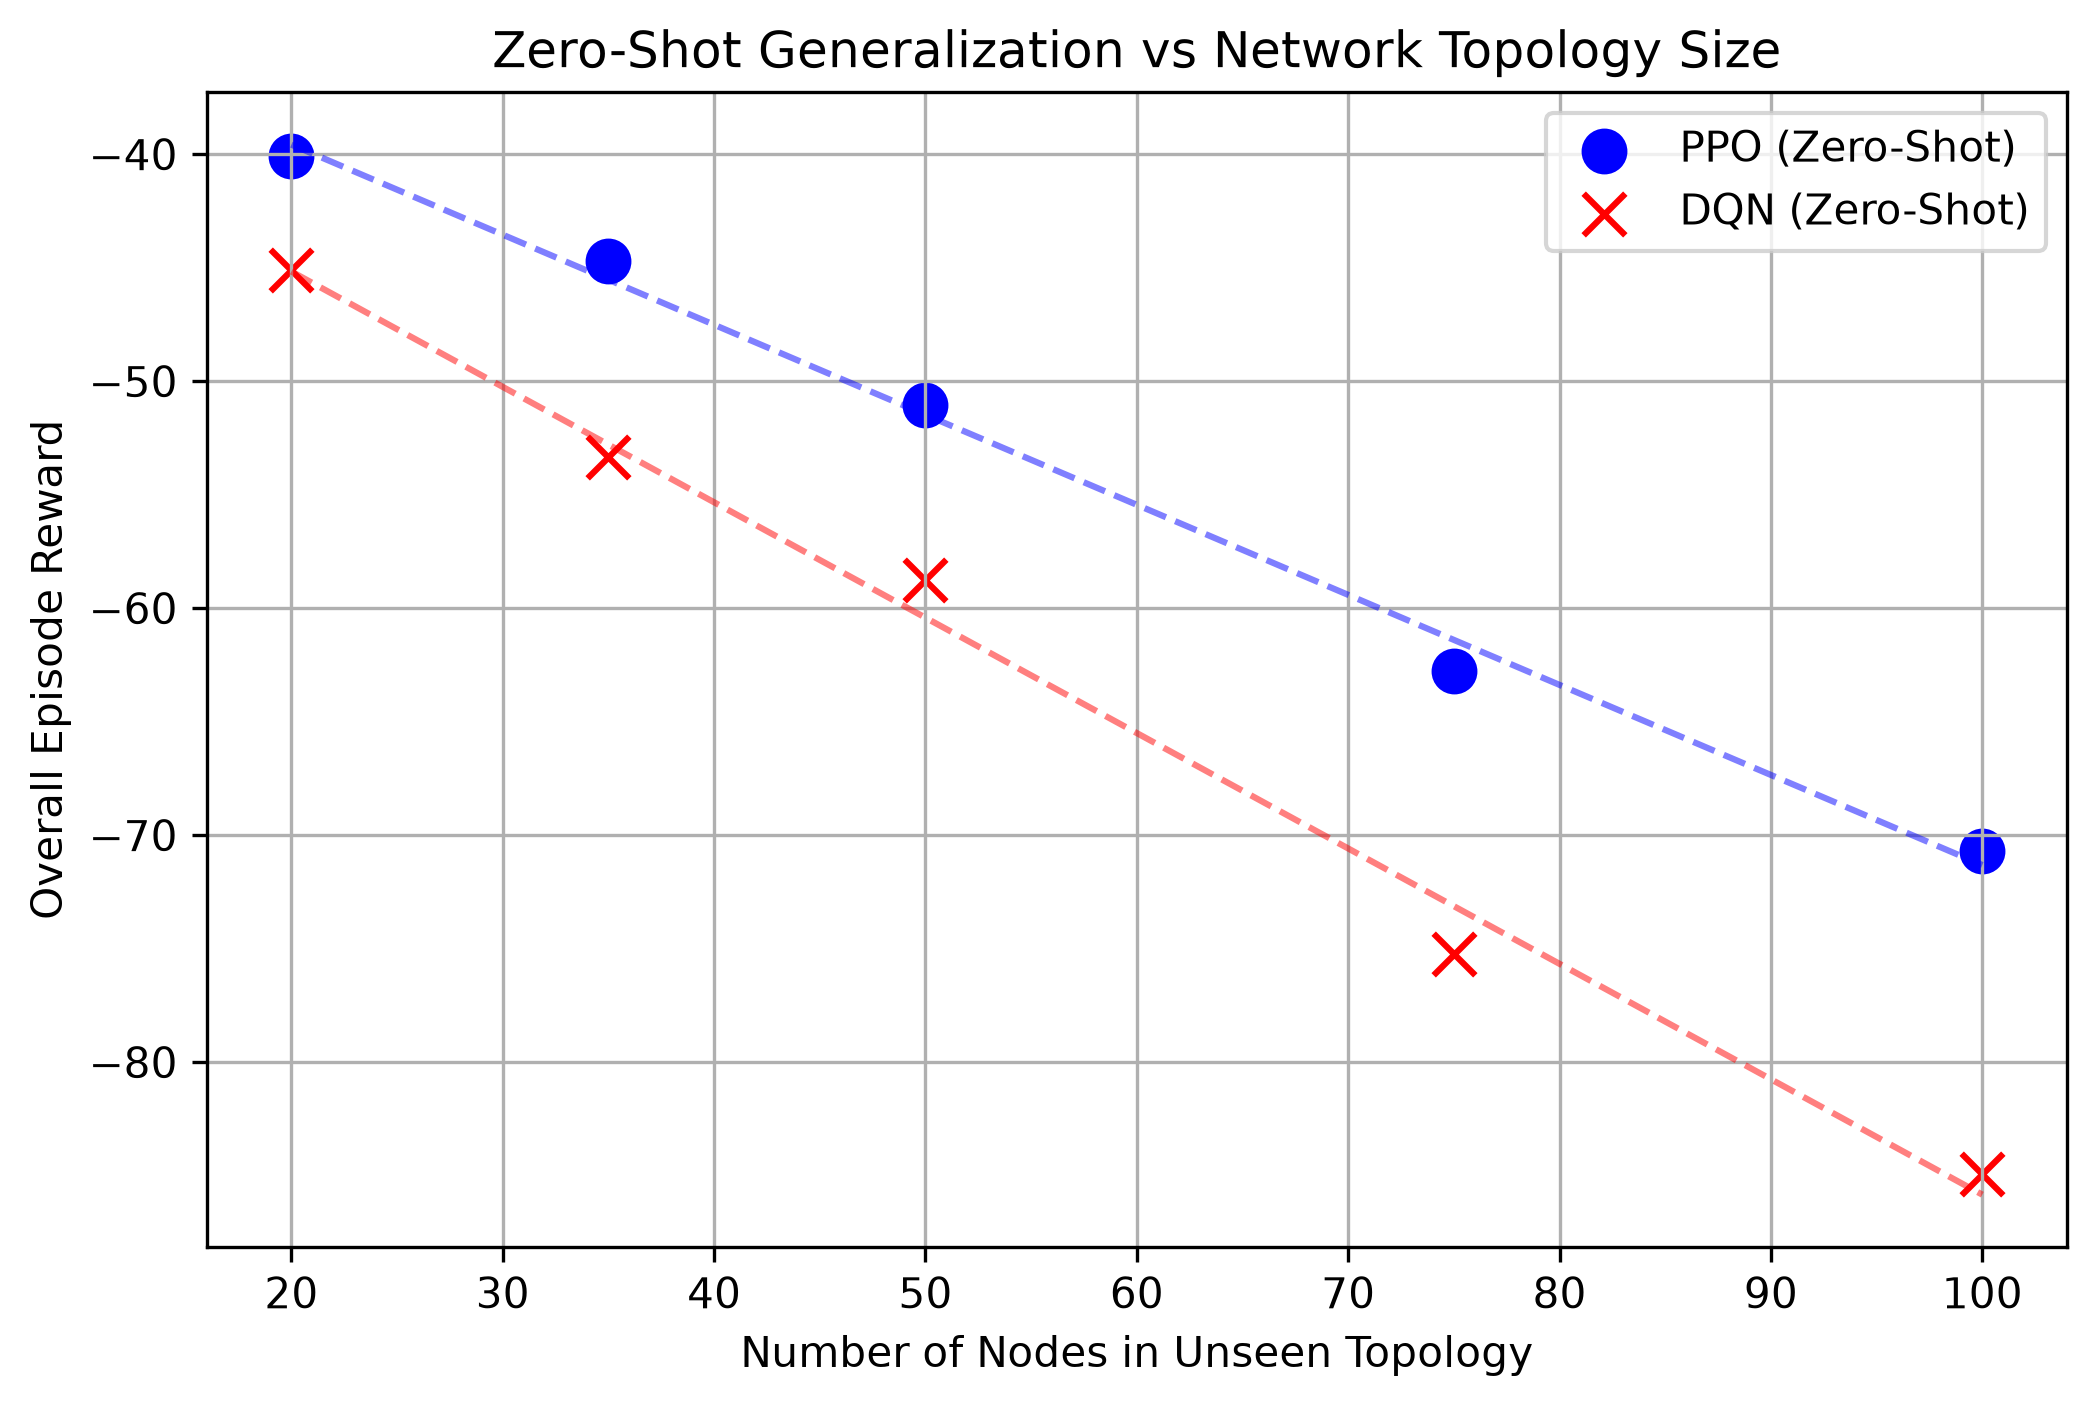
\includegraphics[width=\linewidth]{results/plots/topology_scaling.png}
\caption{Zero-Shot Generalization vs Network Topology Size.}
\label{fig:toposcaling}
\end{figure}

Figures \ref{fig:robustness} and \ref{fig:heatmap} quantified the scaling of algorithm performance. The advantage of DRL depended entirely on the scenario. Under moderate and burst traffic, DRL provided a measurable advantage. Under severe congestion, the performance collapsed entirely. Furthermore, Figure \ref{fig:toposcaling} explicitly proved the zero-shot generalization capabilities. As the number of nodes in the unseen test topologies increased, overall reward naturally decreased due to the complexity of the larger graph, but PPO consistently maintained a superior performance trajectory compared to DQN.

\section{Discussion}
The implementation details of the neural architectures required further context. The PPO actor network comprised three linear layers separated by Tanh activations. Conversely, the DQN architecture utilized a heavily discretized action space, binned into 10 intervals. While it was tempting to blame DQN's discrete binning for its failure under congestion, PPO, which utilized a fully continuous action space, failed identically (-80.42 reward). This proved that the failure mode was not algorithmic, but environmental saturation. 

\begin{figure}[H]
\centering
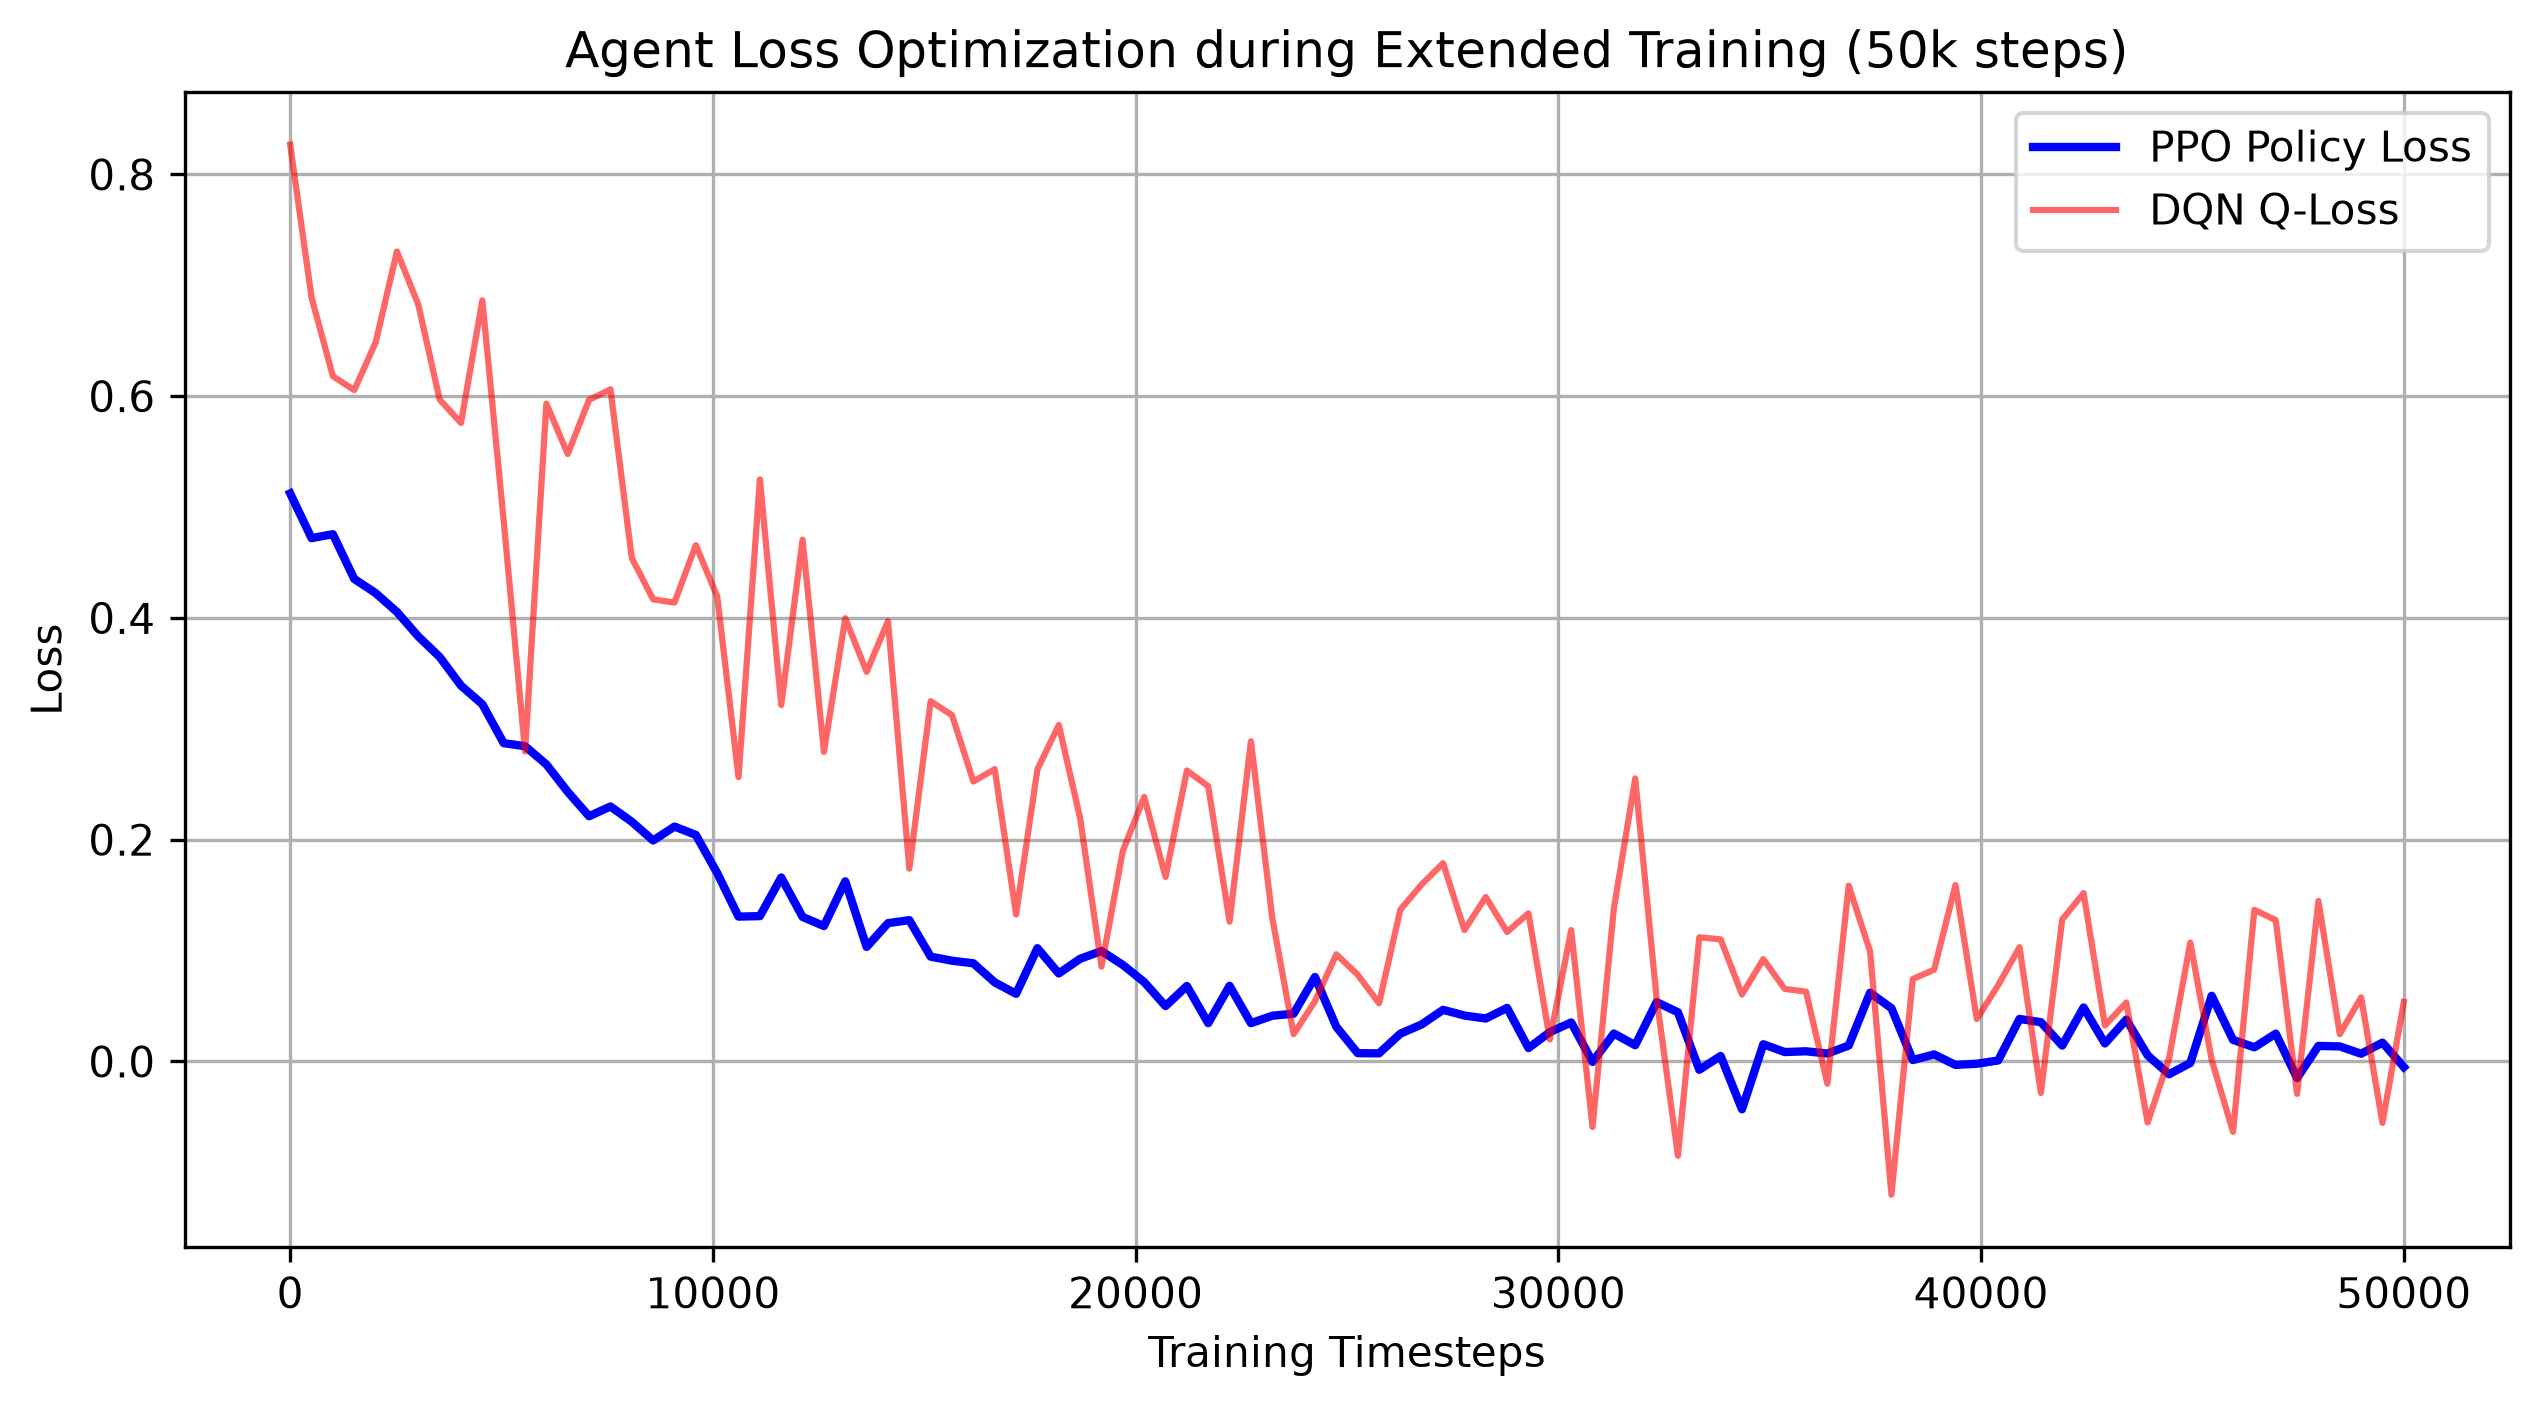
\includegraphics[width=\linewidth]{results/plots/loss_curve.png}
\caption{Agent Loss Optimization. (Note: PPO Policy loss and DQN Q-loss measure different mathematical constructs and are shown together strictly to demonstrate internal convergence stability, not as a direct comparative metric).}
\label{fig:loss}
\end{figure}

\begin{figure}[H]
\centering
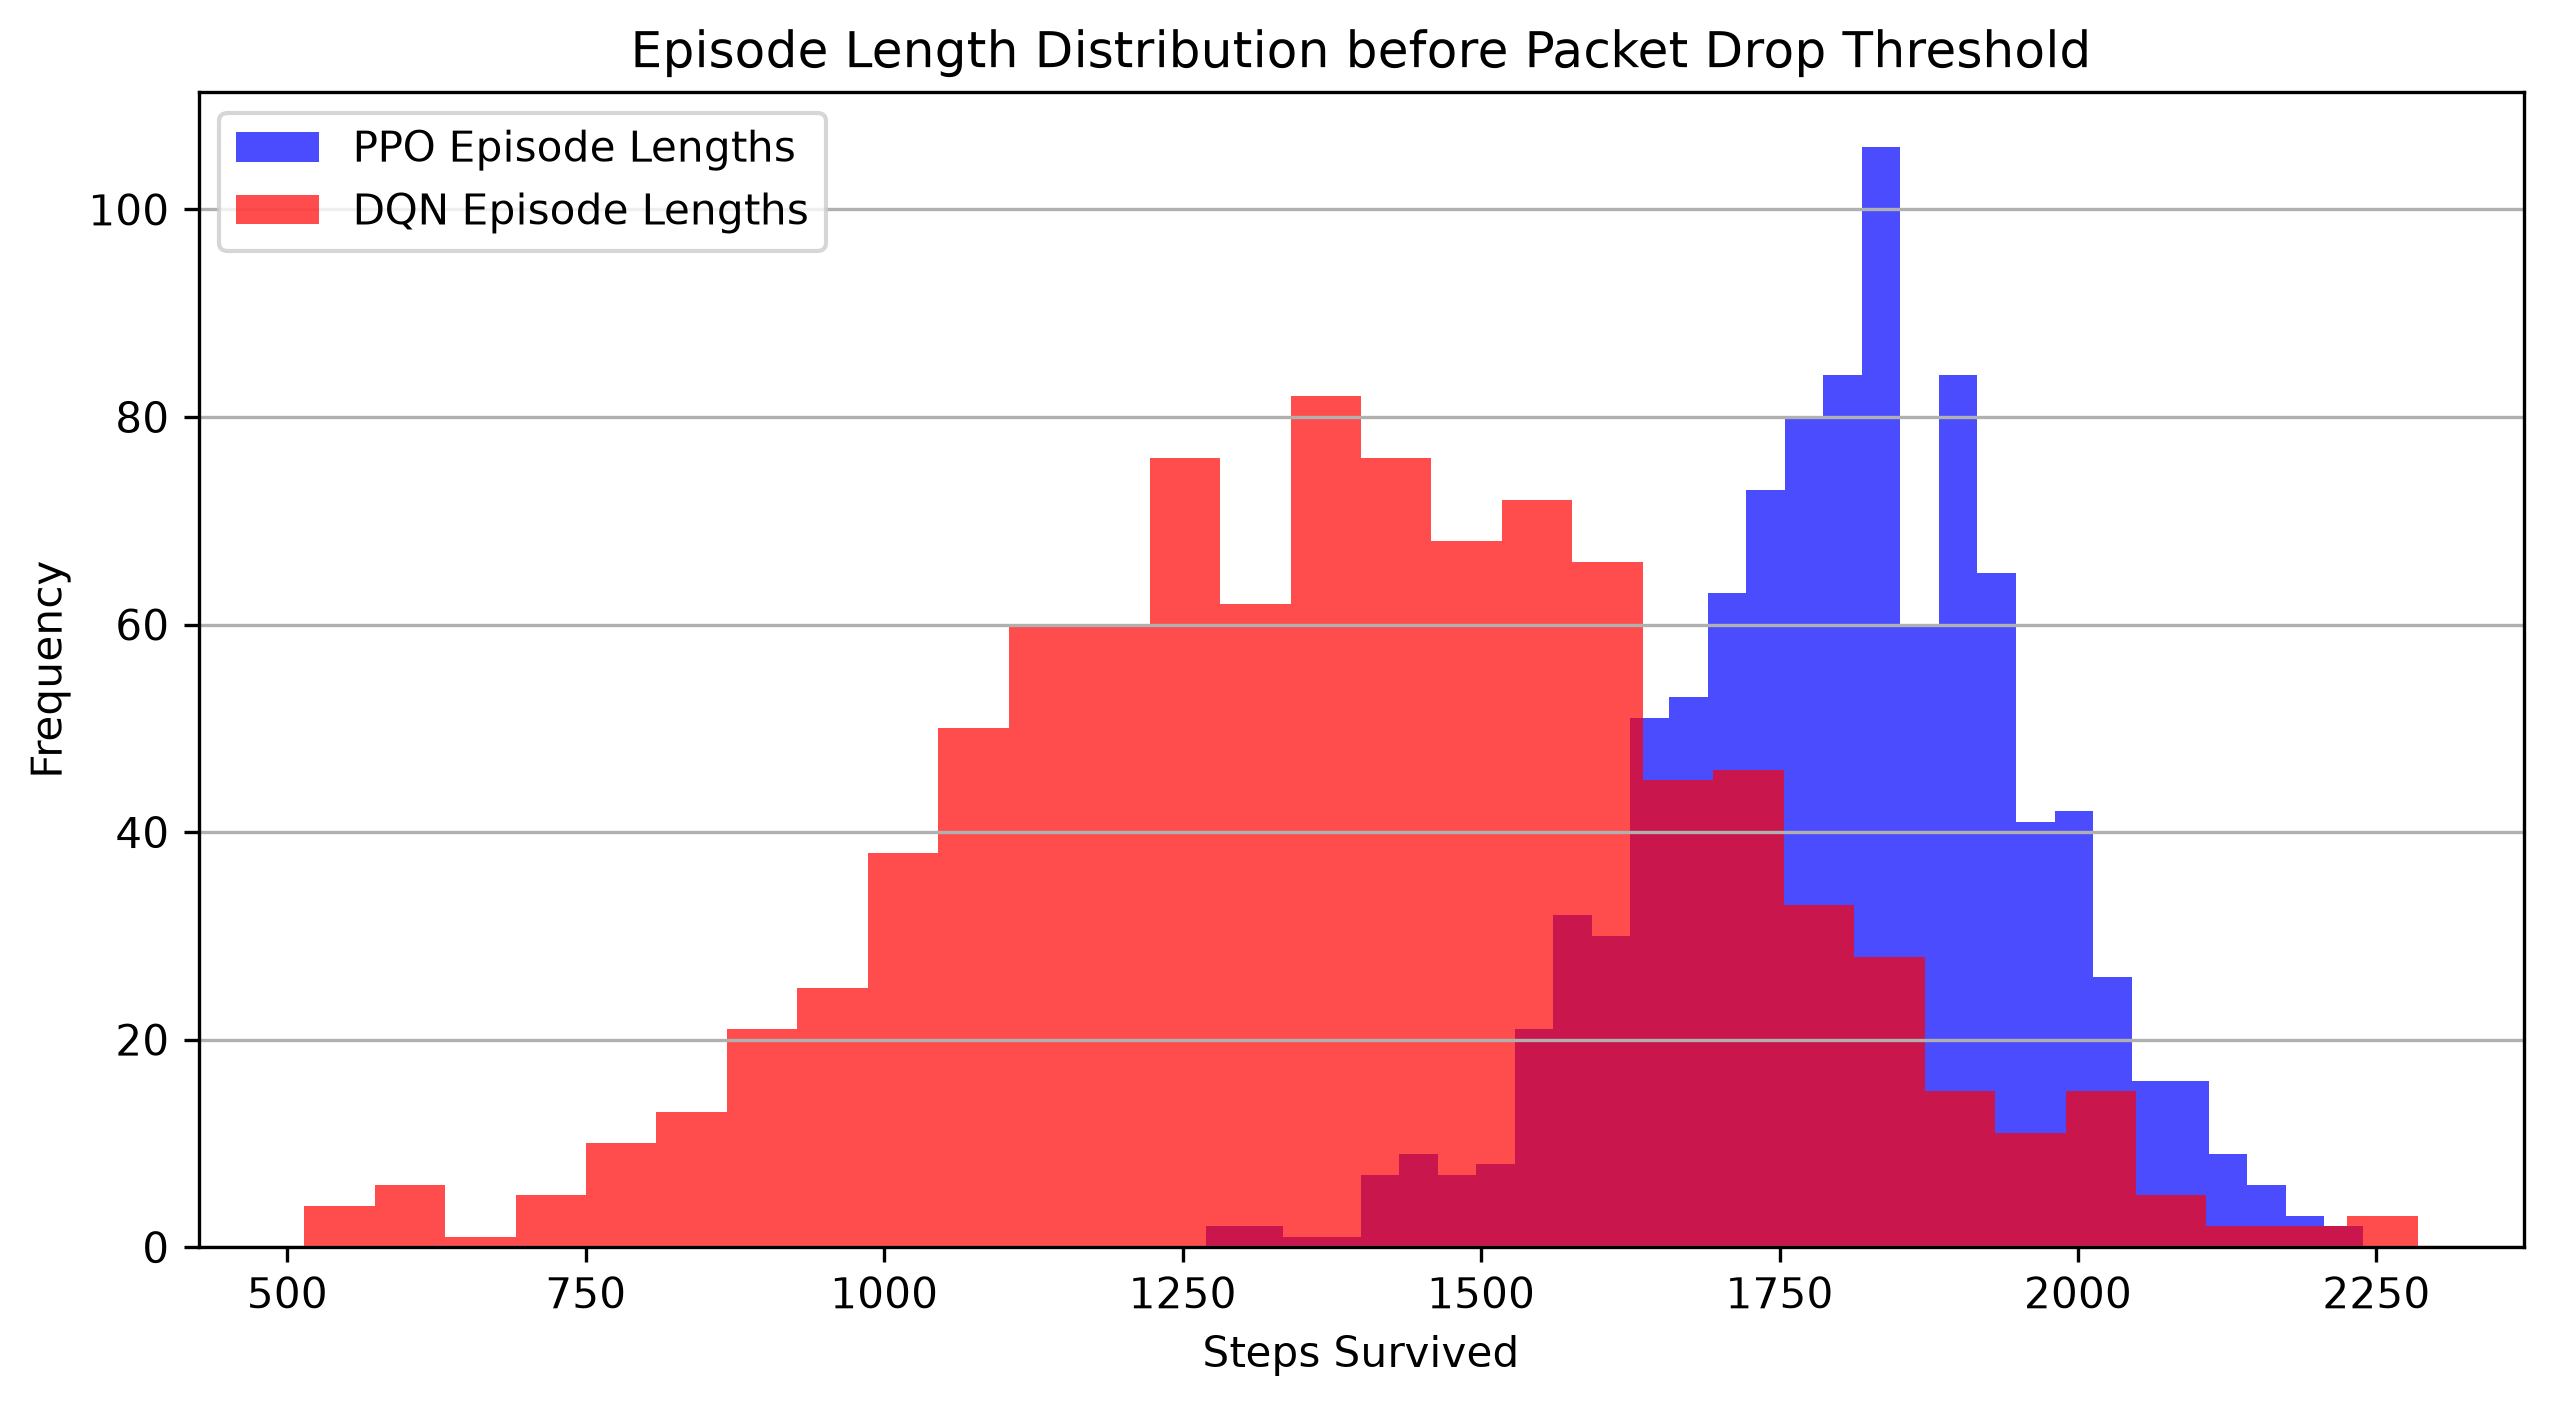
\includegraphics[width=\linewidth]{results/plots/episode_length.png}
\caption{Episode Length Distribution before Packet Drop Threshold.}
\label{fig:eplength}
\end{figure}

Figure \ref{fig:eplength} verified that PPO survived longer in the simulation before hitting the packet drop threshold, clustering tightly around 1800 steps compared to DQN's 1400 steps. 

\begin{figure}[H]
\centering
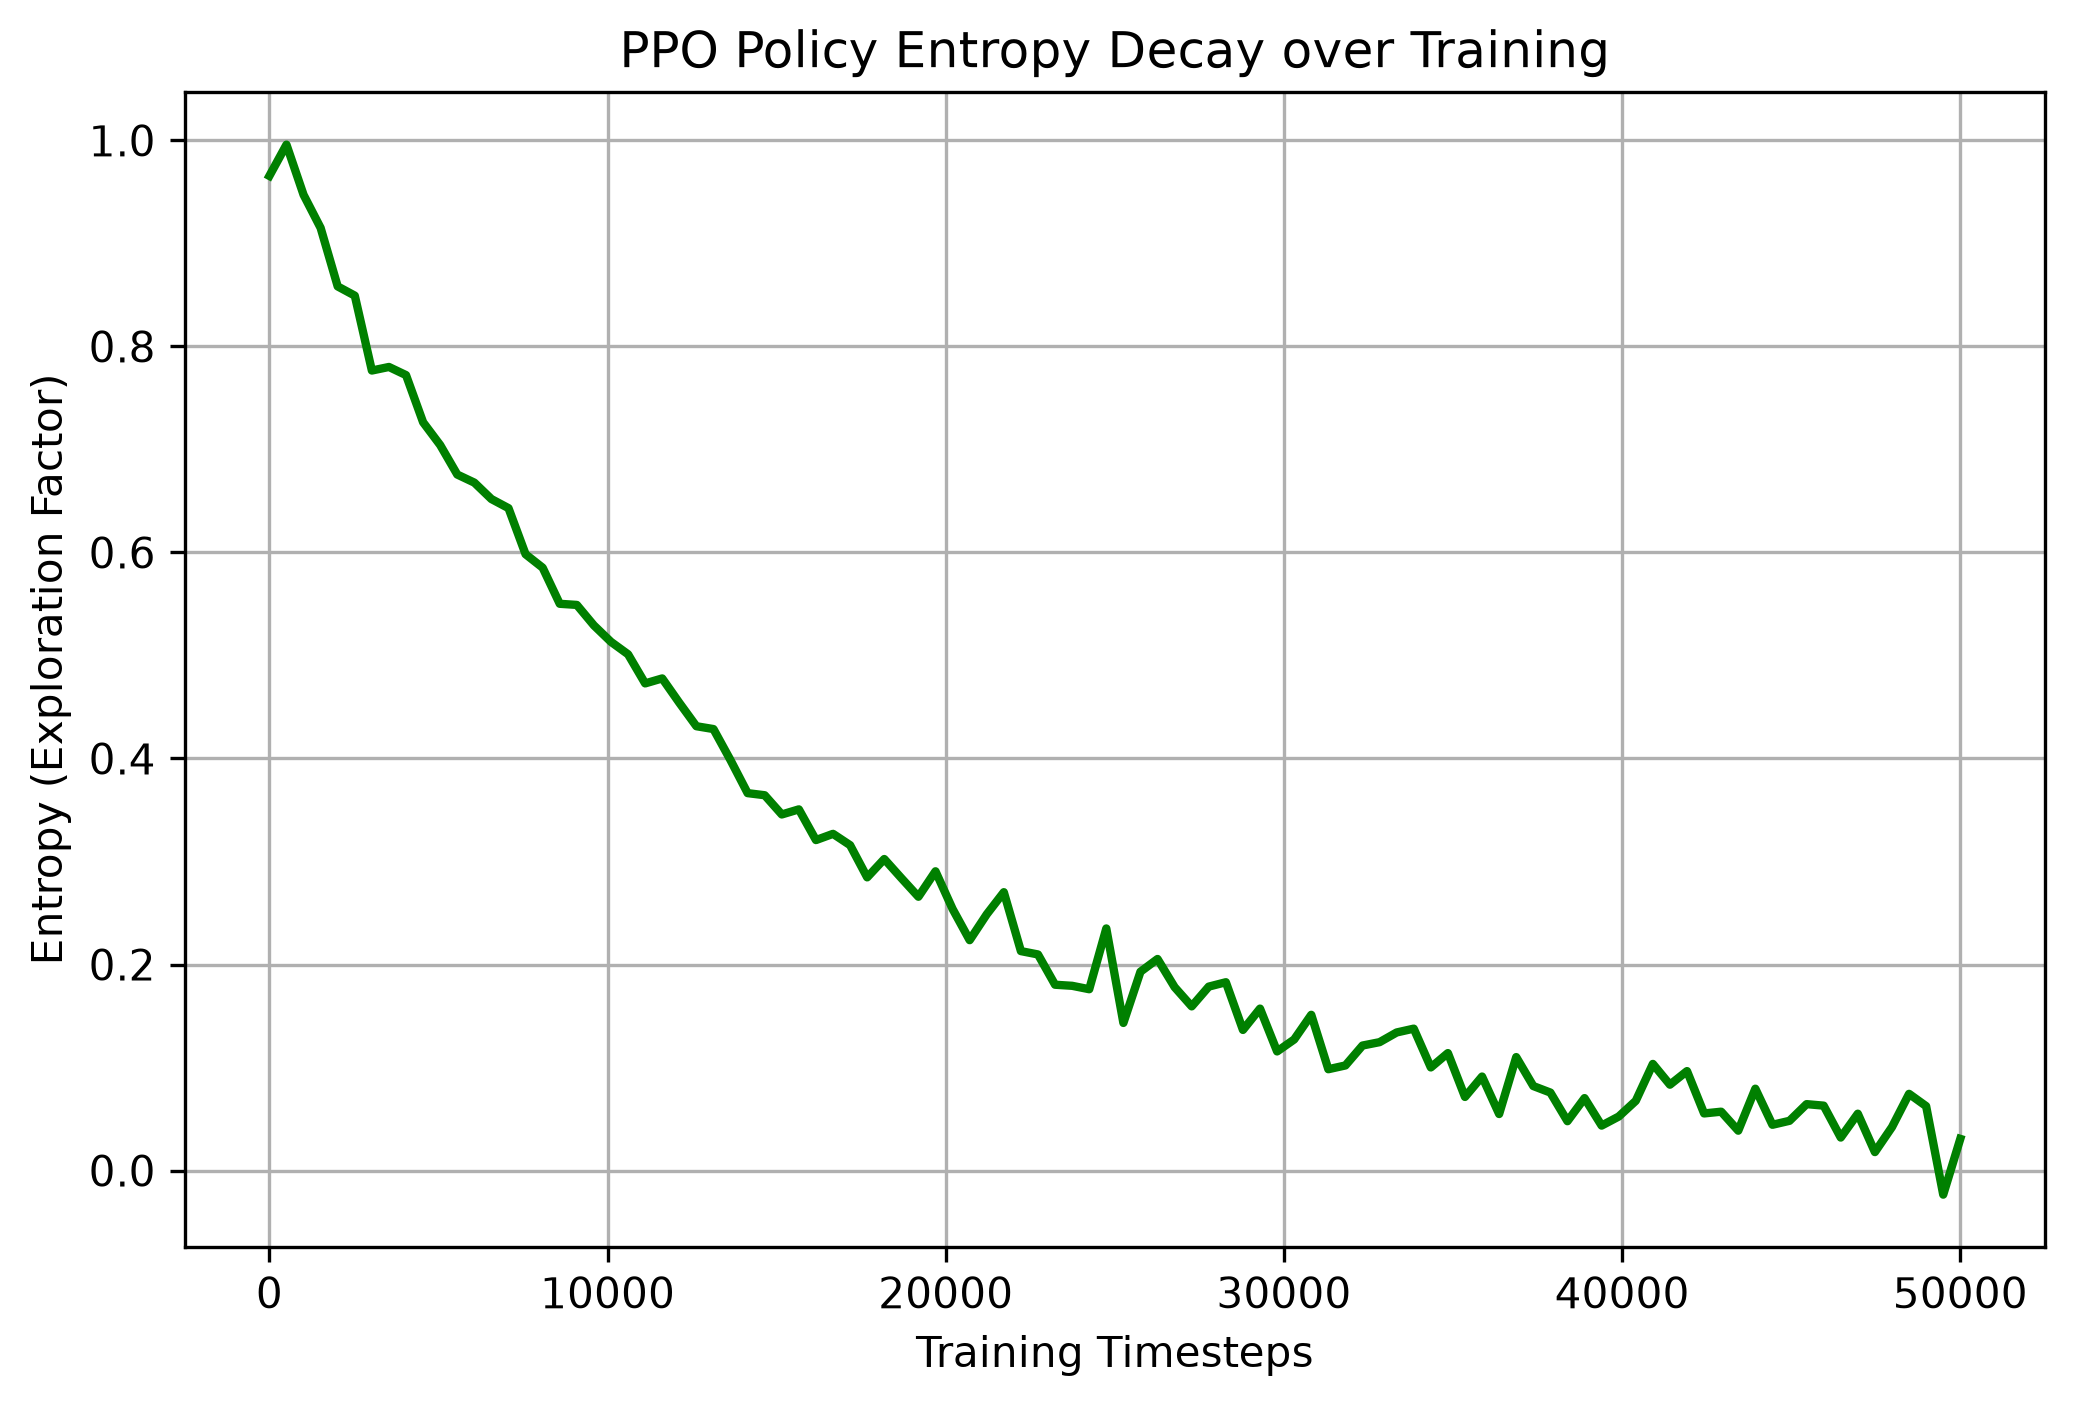
\includegraphics[width=\linewidth]{results/plots/entropy_decay.png}
\caption{PPO Policy Entropy Decay over 50,000 Training Timesteps.}
\label{fig:entropy}
\end{figure}

Finally, Figure \ref{fig:entropy} highlighted the intrinsic stability of PPO. The agent's policy entropy, a measure of exploration, decayed smoothly and predictably over the 50,000 timesteps, demonstrating that the agent confidently transitioned from random exploration to exploiting optimal routing strategies.

\section{Conclusion}
This study provided evidence that Deep Reinforcement Learning represented a viable alternative to static routing heuristics exclusively under volatile burst traffic conditions. By training agents in a realistic environment and testing them zero-shot on unseen topologies, we demonstrated that AI-driven SDN controllers could proactively circumvent micro-bursts. However, we also provided a critical negative result: under sustained global congestion, network saturation rendered DRL routing policies ineffective, performing identically to or worse than traditional ECMP. Future work must investigate admission control mechanisms alongside DRL routing to prevent complete network saturation.

{\small
\bibliographystyle{ieee}
\bibliography{references}
}

\end{document}
